\documentclass[12pt, a4paper]{article}
\usepackage{bookmark}
\usepackage{fullpage} % uniform 1.5 margins
\usepackage[polish]{babel}
\usepackage{polski}
\let\babellll\lll % babel and math shenanigans :/
\let\lll\relax
\usepackage[top=2cm, bottom=4.5cm, left=2.5cm, right=2.5cm]{geometry}  % page customization
\usepackage[T1]{fontenc} % use 8-bit font encoding
\usepackage{amsmath,amsthm,amsfonts,amssymb} % lovely American Mathematical Society packages
\let\mathlll\lll
\let\lll\babellll
\frenchspacing
\usepackage[makeroom]{cancel} % usefull cancelling (slash) command
\usepackage[dvipsnames,table]{xcolor} % colors!!!
\usepackage{float} % stop figures going to the top of the page u stupido by [H] placement
\usepackage{mathtools} % more cool math features
\usepackage{enumitem} % cool enumeration additions
\usepackage{fancyhdr} % fancy headers and footers
\usepackage{mathrsfs} % \mathscr command for cool font
\usepackage{graphicx} % enhanced support for graphics
\usepackage{hyperref} % extensive support for hypertext
\usepackage{theoremref} % refer to theorems using /ref
\usepackage{systeme} % french lib for systems of eq-ns
\usepackage{empheq} % emphasise eq-ns
\usepackage{multicol} % cool columns!
\usepackage{nicematrix} % nice matrices
\usepackage{tikz}  % plots!!
\usepackage{makecell} % cool table cell manipulation
\usepackage{calc} % arithmetic operations on internal counters (e.g. skipping enumeration)
\usepackage{stackengine} % stack engine; stack things on top of things!
\usepackage{diagbox} % table head with diagonal lines
\usepackage{yfonts} % support for old German fonts: gothic, schwabacher, fraktur and baroque
\usepackage{wrapfig} % wrap text around figures
\usepackage{mathdots} % more math dots!
\usepackage[bottom]{footmisc} % some footnote things
\usepackage[justification=centering]{caption} % customize captions in floats
\usepackage{subcaption} % subcaptions for subfigures
\usepackage[all]{nowidow} % avoid widows!
\usepackage{extarrows} % more arrows!
\usepackage{multirow}
\usepackage{amsmath} % fonts for algorithms
\usepackage{algorithm}
\usepackage{algorithmicx} % algorithms, pseudocode
\usepackage[noend]{algpseudocode} % algorithms, pseudocode
\usepackage{soul} % better underline (ul)
\setul{2pt}{.4pt} % set underline to be 2pt below contents

\usepackage{listings}
\usepackage{xcolor}
\lstset { %
    language=C++,
    backgroundcolor=\color{black!5}, % set backgroundcolor
    basicstyle=\footnotesize,% basic font setting
}
\input{insbox} % Floating box tex macro

% change algorithm label
\makeatletter
\renewcommand{\ALG@name}{Algorytm}
\makeatother

\makeatletter
\def\BState{\State\hskip-\ALG@thistlm}
\makeatother

\makeatletter
\algnewcommand{\LineComment}[1]{\Statex \hskip\ALG@thistlm \(\triangleright\) #1}
\makeatother

% equations and figures counted by sections
\counterwithin{equation}{section}
\counterwithin{figure}{section}

\renewcommand\useanchorwidth{T} % https://tex.stackexchange.com/questions/205145/flip-the-underbrace
\renewcommand\theadalign{bc} % table head align - bottom center
\renewcommand\theadfont{\bfseries} % table head font
\renewcommand\theadgape{\Gape[4pt]} % some table spacings ig
\renewcommand\cellgape{\Gape[4pt]}

\widowpenalty10000
\clubpenalty10000

% hypertext config
\hypersetup{
	colorlinks=true,
	citecolor=black,
	filecolor=black,
	linkcolor=black,
	urlcolor=black
}

% rename Rysunek to Rys.
\addto\captionspolish{%
	\renewcommand{\figurename}{Rys.}
}

% make space of width of one text and fill with other
\newcommand{\textover}[3][l]{%
	% #1 is the alignment, default l
	% #2 is the text to be printed
	% #3 is the text for setting the width
	\ensuremath{\makebox[\widthof{#3}][#1]{#2}}%
}

% matrix of type: ... ... ... | ...
\newenvironment{amatrix}[1]{%
	\begin{bNiceArray}{*{#1}{c}|c}
	}{%
	\end{bNiceArray}
}

% use boondox font on \mathds command
\DeclareMathAlphabet{\mathds}{U}{BOONDOX-ds}{m}{n}

\setlength{\parindent}{0.0in}
\setlength{\parskip}{0.05in}

% theorems with * are not numbered
\newtheorem{axiom}{Aksjomat}[section]
\newtheorem{theorem}{Twierdzenie}[section]
\newtheorem{defi}{Definicja}[section]
\newtheorem{corollary}{Wniosek}[theorem]
\newtheorem*{corollary*}{Wniosek}
\newtheorem{lemma}{Lemat}[section]
\newtheorem*{lemma*}{Lemat}
\newtheorem{excercise}{Zadanie}[section]
\newtheorem*{excercise*}{Zadanie}
\newtheorem*{example}{Przykład}
\newtheorem*{note}{Uwaga}
\newtheorem*{przp}{Przypomnienie}
\newtheorem{prop}{Własność}[section]
\newtheorem{fact}{Fakt}[section]
\newtheorem{algo}{Algorytm}[section]
\newtheorem{obs}{Obserwacja}

% things needed for my basic template to work
\newcommand\person{M. Okurowski, M. Słupczyński, J. Żuchowski}
\newcommand\depart{Wydział MiNI PW}

% slightly higher fbox? dont remember
\newcommand*\widefbox[1]{\fbox{\hspace{2em}#1\hspace{2em}}}

% footer and header setup
\pagestyle{fancyplain}
\headheight 35pt
\lhead{AiSD 2, \depart}
%\chead{\textbf{\Large \dtype}\\\leftmark}
%\rhead{\course \\ \today}
\lfoot{}
\cfoot{}
\rfoot{\small\thepage}
\headsep 1.5em

% custom command for putting things on top of = sign
\newcommand{\myeq}[2][=]{\mathrel{\overset{#2}{#1}}}

% math sets defined
\newcommand\N{\ensuremath{\mathbb{N}}}
\newcommand\R{\ensuremath{\mathbb{R}}}
\newcommand\Z{\ensuremath{\mathbb{Z}}}
\newcommand\Q{\ensuremath{\mathbb{Q}}}
\newcommand\C{\ensuremath{\mathbb{C}}}
\renewcommand\d{\ensuremath{\mathrm{d}}}
\newcommand{\val}[0]{\mathrm{val}}

% force \limits after \lim, old lim available as \svlim
\let\svlim\lim\def\lim{\svlim\limits}
% remove those ugly ass characters ew
\let\Re\relax 
\let\Im\relax
% \arccot is something wrong
\let\arccot\relax

% define my own operators
\DeclareMathOperator{\Re}{Re}
\DeclareMathOperator{\Im}{Im}
\DeclareMathOperator{\Arg}{Arg}
\DeclareMathOperator{\diag}{diag}
\DeclareMathOperator{\rz}{rz}
\DeclareMathOperator{\tr}{tr}
\DeclareMathOperator{\arccot}{arccot}

\usepackage{cutwin} % cut windows in paragraphs
\usepackage{pgfplots} % even better plots!!!
\pgfplotsset{compat=1.17}
\usetikzlibrary{matrix,calc,patterns,angles,quotes}
\usetikzlibrary{arrows.meta, intersections, fillbetween,babel}

% you know \cancelto? yea its always cancelling upwards, there is no \bcancelto, so here it is
\makeatletter
% #1, #2 offset of label   #6 extra width to clear arrowhead
% #3, #4 vector direction  #7 superscript label style
% #5 vector width          #8 superscript label
\def\cantox@vector#1#2#3#4#5#6#7#8{%
	\dimen@.5\p@
	\setbox\z@\vbox{\boxmaxdepth.5\p@
		\hbox{\kern-1.2\p@\kern#1\dimen@$#7{#8}\m@th$}}%
	\ifx\canto@fil\hidewidth  \wd\z@\z@ \else \kern-#6\unitlength \fi
	\ooalign{%
		\canto@fil$\m@th \CancelColor
		\vcenter{\hbox{\dimen@#6\unitlength \kern\dimen@
				\multiply\dimen@#4\divide\dimen@#3 \vrule\@depth\dimen@\@width\z@
				\vector(#3,-#4){#5}%
		}}_{\raise-#2\dimen@\copy\z@\kern-\scriptspace}$%
		\canto@fil \cr
		\hfil \box\@tempboxa \kern\wd\z@ \hfil \cr}}
\def\bcancelto#1#2{\let\canto@vector\cantox@vector\cancelto{#1}{#2}}
\makeatother

% some cute colors
\definecolor{highlight}{HTML}{FFFEEC}
\definecolor{highlight2}{HTML}{FAFFEC}

% \highlight[<color>]{<stuff>}
\newcommand{\highlight}[2][highlight]{\mathchoice%
	{\colorbox{#1}{$\displaystyle#2$}}%
	{\colorbox{#1}{$\textstyle#2$}}%
	{\colorbox{#1}{$\scriptstyle#2$}}%
	{\colorbox{#1}{$\scriptscriptstyle#2$}}}%

% Default plot config
\pgfplotsset{every axis/.append style ={
	width=1\linewidth,
	axis equal image,
	axis x line=center,
	axis y line=center,
	xlabel style={at={(current axis.right of origin)},anchor=north},
	ylabel style={at={(current axis.above origin)},anchor=east},
	trig format plots=rad,
	unbounded coords=jump,
	xlabel={$x$},
	ylabel={$y$},
}}

% some cute open and closed points
\tikzset{
	circ/.style={circle,fill=white,draw,inner sep=1.5pt,outer sep=0pt, fill opacity=1},
	poin/.style={circ,fill=#1,draw=#1,},
	poin/.default=black,
}

\newcounter{daggerfootnote}
\newcommand*{\daggerfootnote}[1]{%
	\setcounter{daggerfootnote}{\value{footnote}}%
	\renewcommand*{\thefootnote}{\fnsymbol{footnote}}%
	\footnote[2]{#1}%
	\setcounter{footnote}{\value{daggerfootnote}}%
	\renewcommand*{\thefootnote}{\arabic{footnote}}%
}

\let\originalleft\left
\let\originalright\right
\renewcommand{\left}{\mathopen{}\mathclose\bgroup\originalleft}
\renewcommand{\right}{\aftergroup\egroup\originalright}

\newcommand{\pleq}{\mathrel{\scalebox{0.75}{+{=}}}}
\newcommand{\mieq}{\mathrel{\scalebox{0.75}{-{=}}}}
\newcommand{\pp}{\scalebox{0.75}{++}}
\newcommand{\mm}{\scalebox{0.75}{$--$}}
\usepackage{xspace}
\newcommand{\true}{\textsf{true\xspace}}
\newcommand{\false}{\textsf{false\xspace}}
\usepackage{lmodern}

\captionsetup[table]{font=small}
\captionsetup[figure]{font=small}

\begin{document}

\begin{titlepage}
    \begin{center}
        \vspace*{1cm}

        \Huge

        \textbf{Algorytmy i Struktury Danych 2}

        \vspace{1.5cm}

        \LARGE

        \textbf{Michał Okurowski}

        \vfill  

        \vspace{0.8cm}

        
\includegraphics[width=0.4\textwidth]{data/university.png}

        Wydział Matematyki i Nauk Informacyjnych\\
        Politechnika Warszawska\\
    \end{center}
\end{titlepage}

\tableofcontents
\pagebreak

\section{Programowanie dynamiczne}
Programowanie dynamiczne ma zastosowanie w problemach wykazujących 
własność \textbf{optymalnej podstruktury} –
to znaczy, kiedy optymalne rozwiązanie problemu 
łatwo jest uzyskać znając optymalne rozwiązania podproblemów. 

\subsection{Znajdowanie najdłuższego podciągu rosnącego}
Rozważmy następujący problem: 
\begin{itemize}
	\item[] \textbf{Dane:} Pewien ciąg $c = c_1,c_2, \ldots, c_n$
	\item[] \textbf{Szukane:} Dowolny najdłuższy podciąg 
	$c_{i_1},c_{i_2},\ldots, c_{i_k}$ ciągu $c$, taki, że
	$i_1 < i_2 < \ldots < i_k$ oraz $c_{i_1} < c_{i_2} < \ldots < c_{i_k}$.    
\end{itemize}

Przykładowo, dla wejściowego ciągu $(3, 1, 8, 2, 5)$ odpowiedzią będzie
ciąg $(1, 8, 5)$.

W pierwszym kroku rozwiązywania problemów programowania dynamicznego, szukamy
odpowiedniego podproblemu. Dla ułatwienia, zareprezentujmy ciąg jako 
graf skierowany $G$, w którym wierzchołkami są elementy ciągu $c$ oraz 
istnieje krawędź z wierzchołka $c_i$ do wierzchołka $c_j$ jeśli $x < y$
oraz $i < j$. 
Opisany graf dla powyższego przykładu wygląda tak jak na rysunku
\ref{fig:example111_max_length}.

\begin{figure}[H]
	\centering
	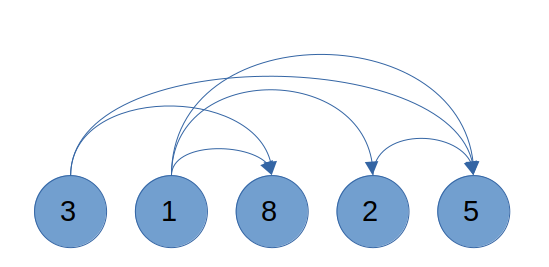
\includegraphics[width=0.4\textwidth]{data/prblm1_ex_graph.png}
	\caption{ }
	\label{fig:example111_max_length}
\end{figure}

Uprośćmy tymczasowo analizowany problem do problemu znajdowania 
długości najdłuższego rosnącego podciągu. Utwórzmy tablicę \textit{T} 
(numerujemy od 1), w której na indeksie $i$ 
będziemy przechowywać długość najdłuższego podciągu, dla którego $c_i$
jest jego ostatnim elementem. Przypuśćmy, że wypełniliśmy tablicę 
$T$ do ($i-1$)-tego elementu.
Wtedy aby poznać wartość na $i$-tym indeksie wystarczy przeanalizować 
wszystkie te wierzchołki w grafie $G$ które mają skierowaną krawędź na
$i$-ty wierzchołek.

\begin{figure}[H]
	\centering
	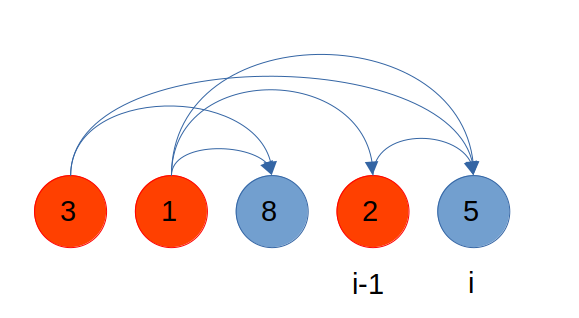
\includegraphics[width=0.4\textwidth]{data/prblm1_ex_graph2.png}
	\caption{  }
	\label{fig:example112_max_length}
\end{figure}

Niech $I$ to zbiór indeksów wszystkich elementów ciągu $c$, które są 
mniejsze niż $c_i$, wtedy 
\[T[i]=\max\limits_{j \in I}\{T[j]\} + 1.\]

Jeśli wypełnimy całą tablicę $T$ wg. powyższej procedury, odpowiediedzą
będzie maksymalny element tablicy $T$.

\begin{algorithm}[H]
	\caption{Znajdowanie najdłuższego rosnącego podciągu.}\label{MaxIncreasingSubseqenceLength}
	\begin{algorithmic}[1]
		\Procedure{MaxIncreasingSubseqenceLength($c = c_1,c_2, \ldots, c_n$)}{}
		\State Utwórz tablicę $n$-elementową $T$
		\State Ustaw wartość każdej komórki tablicy $T$ na $1$
		\State $i \gets 2$
		\While{$i \leq n$}
		\State $j \gets 1$
		\While{$j \leq i - 1$}
		\If{$c_i \geq c_j$ } 
		\textbf{continue}
		\EndIf
		\If{$T[i] \leq T[j] + 1$ } 
		\State $T[j] \gets T[i]$
		\EndIf
		\EndWhile
		\EndWhile
		\State \Return $\max\limits_{1 \leq i \leq n}\{T[i]\}$
		\EndProcedure
	\end{algorithmic}
\end{algorithm}

Złożoność czasowa powyszego rozwiązania jest rzędu $n^2$. 

Powyższy algorytm można bardzo łatwo zmodyfikować w taki sposób, aby
możliwym było zwrócenie podciągu stanowiącego rozwiązanie (problem pierwotny).
Wystarczy utworzyć tablicę $P$, która na indeksie $i$
będzie zapisywać indeks ostatniego elementu, który spełnił 
warunek $T[i] \leq T[j] + 1$. Ustalmy, że $-1$ będzie oznaczało, że 
takiego elementu nie ma (tzn. $c_i$ jest pierwszym elementem podciągu).

\begin{algorithm}[H]
	\caption{Znajdowanie najdłuższego rosnącego podciągu.}\label{MaxIncreasingSubseqence}
	\begin{algorithmic}[1]
		\Procedure{MaxIncreasingSubseqence($c = c_1,c_2, \ldots, c_n$)}{}
		\State Utwórz tablicę $n$-elementową $T$
		\State Ustaw wartość każdej komórki tablicy $T$ na $1$
		\State Utwórz tablicę $n$-elementową $P$
		\State Ustaw wartość każdej komórki tablicy $P$ na $-1$
		\State $i \gets 2$
		\While{$i \leq n$}
		\State $j \gets 1$
		\While{$j \leq i - 1$}
		\If{$c_i \geq c_j$ } 
		\textbf{continue}
		\EndIf
		\If{$T[i] \leq T[j] + 1$ } 
		\State $T[j] \gets T[i]$
		\State $P[i] \gets j$
		\EndIf
		\EndWhile
		\EndWhile
		\State $m = \max\limits_{1 \leq i \leq n}\{T[i]\}$ 
		\State Utwórz tablicę $m$-elementową $A$ reprezentującą
		kolejne wartości szukanego podciągu
		\State $i \gets m$
		\State $j \gets$ indeks elementu o wartości $m$
		\While{$i \geq 1$}
		\State $A[i] \gets c_j$
		\State $j \gets P[j]$
		\State $i \gets i - 1$
		\EndWhile
		\State \Return $A$
		\EndProcedure
	\end{algorithmic}
\end{algorithm}

\subsection{Problem wydawania reszty}
Rozważmy następujący problem:
\begin{itemize}
	\item[] \textbf{Dane:} Nominały monet $n_1$, $n_2$, 
	$\ldots$, $n_k \in \mathbb{N}$ oraz kwota $K \in \mathbb{N}$
	\item[] \textbf{Szukane:} Ciąg liczb naturalnych $a = a_1$, $a_2$,
	$\ldots$ $a_k$ taki, że 
	\[\sum\limits_{i=1}^{k} a_in_i = K \text{ oraz suma } 
	\sum\limits_{i=1}^{k} a_i
	\text{ jest najmniejsza możliwa,}\]
	innymi słowy, szukamy sposobu na wydanie kwoty $K$, z użyciem
	jak najmniejszej liczby monet.
\end{itemize}

Na początek zaobserwujmy, że jeśli $a = a_1$, $a_2$,
$\ldots$ $a_k$ to rozwiązanie optymalne powyższego problemu, to 
zmniejszenie $a_i \geq 1$ ($i \in [k]$) o $1$, powinno 
zaskutkować powstaniem rozwiązania problemu dla kwoty $K - n_i$.
To stwierdzenie musi być prawdziwe, bo inaczej moglibyśmy
skonstruować rozwiązanie o mniejszej liczbie monet
niż optymalne co jest sprzeczne.

Przykładowo, dla $K = 13$ i nominałów $(1, 2, 5)$, optymalnym
rozwiązaniem jest ciąg $(1, 1, 2)$. Wtedy ciąg $(0, 1, 2)$
jest optymalnym rozwiązaniem dla $K = 12$, 
$(1, 0, 2)$ jest optymalnym rozwiązaniem dla $K = 11$ oraz
$(1, 1, 1)$ dla $K = 8$.

Z powyższego stwierdzenia wynika, że otrzymanie optymalnego 
rozwiązania dla kwoty $K$ jest możliwe po przeanalizowaniu 
\textit{wszystkich} optymalnych rozwiązań dla kwot $K - n_i$,
co oznacza że udało nam się znaleźć optymalną podstrukturę.

Tak samo jak w przypadku problemu znajdowania najdłuższego 
podciągu rosnącego, rozważmy uproszczoną wersję problemu, 
w której interesować nas będzie nie ciąg $a$, ale 
liczba monet w optymalnym rozwiązaniu. 

Zdefiniujmy tablicę $T$ (indeksowaną od $0$) jako 
tablicę rozmiaru $K + 1$, w której komórka $T[i]$ ($i \in {0, 1, \ldots, K}$)
przechowuje liczbę monet potrzebną do optymalnego wydania kwoty równej $i$.
Z powyższych rozważań
wiadomo, że jeśli tablica jest wypełniona do $(i-1)$-tego
elementu ($i \in {0, 1, \ldots, K}$) włącznie, to 
\begin{equation}
	T[i] = \min_{1 \leq j \leq k}\{T[i - n_j]\} + 1,
	\label{eq:min_change_making_relation}
\end{equation}
ponadto przy takiej definicji tablicy, możemy przyjąć, że $T[0] = 0$.

Na koniec zauważmy, że w badanym problemie
istnieją dane wejściowe, dla których nie 
istnieje rozwiązanie (w szczególności szukane rozwiązanie optymalne),
np. nie możemy wydać $K=3$ dla nominałów $(2, 4)$. 
Aby ułatwić zapis rozwiązania jak i wykrywanie sytuacji, w których
ono nie istnieje, każda komórka tablicy $T$ będzie inicjowana
wartością $\infty$. Jeśli po wykonaniu się algorytmu, $T[K] = \infty$
możemy zwrócić informację, że rozwiązanie nie istnieje.

\begin{algorithm}[H]
	\caption{Znajdowanie liczby monet optymalnego 
		rozwiązania w problemie wydawania reszty.}\label{MinCoinsCountChangeMaking}
	\begin{algorithmic}[1]
		\Procedure{MinCoinsCountChangeMaking($n_1,n_2, \ldots, n_k \in \mathbb{N}$, 
			$K \in \mathbb{N}$)}{}
		\State Utwórz tablicę $(K+1)$-elementową $T$
		\State Ustaw wartość każdej komórki tablicy $T$ na $\infty$
		\State $T[0] = 0$
		\For{$i = 1, 2, \ldots K$}
		\For{$j = 1, 2, \ldots k$}
		\If{$i < n_j$} \textbf{continue}
		\EndIf
		\State $c = T[i - n_j] + 1$
		\If{$c < T[i]$} $T[i] \gets c + 1$
		\EndIf
		\EndFor
		\EndFor
		\If{$T[K] = \infty$} \textbf{return} \textit{null}
		\EndIf
		\State \textbf{return} \textit{T[K]}
		\EndProcedure
	\end{algorithmic}
\end{algorithm}

Powyższy algorytm ma złożoność pamięciową rzędu $K$ oraz czasową $K\cdot k$. 
Gdybyśmy chcieli ten sam problem rozwiązać rekurencyjną metodą otrzymalibyśmy
złożność czasową rzędu $2^K$, przez rozwiązywanie tych samych podproblemów kilkukrotnie.

Aby rozwiązać problem pierwotny, podobnie jak w znajdowaniu najdłuższego
podciągu rosnącego, utworzymy tablicę $P$ o długości $K+1$,
która będzie przechowywać w komórce o indeksie $i \in \{0, 1, \ldots K\}$, indeks $j$
nominału, takiego, że zależność \eqref{eq:min_change_making_relation}
będzie prawdziwa.

\begin{algorithm}[H]
	\caption{Znajdowanie liczby monet optymalnego 
		rozwiązania w problemie wydawania reszty.}\label{ChangeMaking}
	\begin{algorithmic}[1]
		\Procedure{ChangeMaking($n_1,n_2, \ldots, n_k \in \mathbb{N}$, 
			$K \in \mathbb{N}$)}{}
		\State Utwórz tablicę $(K+1)$-elementową $T$
		\State Ustaw wartość każdej komórki tablicy $T$ na $\infty$
		\State Utwórz tablicę $(K+1)$-elementową $P$
		\State $T[0] \gets 0$
		\For{$i = 1, 2, \ldots K$}
		\For{$j = 1, 2, \ldots k$}
		\If{$i < n_j$} \textbf{continue}
		\EndIf
		\State $c = T[i - n_j] + 1$
		\If{$c < T[i]$} 
		\State $T[i] \gets c + 1$
		\State $P[i] \gets j$
		\EndIf
		\EndFor
		\EndFor
		\If{$T[K] = \infty$} \textbf{return} \textit{null}
		\EndIf
		
		\State Utwórz tablicę $T[K]$-elementową $A$ reprezentującą
		kolejne wartości ciągu.
		\State $i \gets K$
		\While{$i > 0$}
		\State $A[P[i]] \gets A[i] + 1$
		\State $i \gets i - n_{P[i]}$
		\EndWhile
		\State \textbf{return} A
		\EndProcedure
	\end{algorithmic}
\end{algorithm}

\subsection{Skreślanie ciągów}
\section{Programowanie dynamiczne -- Zadania}
\subsection{Zadanie 1 -- Szukanie podzbioru o zadanej sumie elementów}
\textbf{Treść: } Zaprojektuj algorytm, który dla zadanego zbioru 
liczb naturalnych $S$ i liczby naturalnej $N$ rozstrzygnie,
czy $S$ zawiera podzbiór o sumie równej $N$ w czasie $O(N |S|)$.

Wskazówka: wyznacz wszystkie możliwe sumy podzbiorów zbioru $S$

\textbf{Rozwiązanie: }

Niech $S = \{s_0, s_1, \dots, s_{|S| - 1}\}$ to zbiór wejściowy, oraz 
niech $N$ to liczba, dla której sprawdzimy czy istnieją elementy, które się do niej sumują.

Niech $T$ to tablica dwuwymiarowa o wymiarach $|S|$ na $N + 1$, przyjmująca wartości 
\textit{True} lub \textit{False} w każdej komórce tablicy $T$.
Komórka tablicy $T[i, j]$ odpowiada na pytanie, czy da się otrzymać 
sumę równą $i$ z $j$-elementowego podzbioru $\{s_1, s_2, \dots, s_j\} \subseteq S$.

Algorytm polega na uzupełnianiu kolejnych wierszy tablicy.
Najpierw rozważamy problem oparty na zbiorze $\{s_1\}$. 
Nastepnie aby otrzymać rozwiązanie dla $\{s_1, s_2\}$, wystarczy
od każdej komórki przechowującej $T$ przemieścić się o $s_2$ komórek w prawo
i zmienić wartość na $T$ i tak do momentu uzupełnienia tablicy $T$.

Po uzupełnieniu $T$ odpowiedzią na zadane pytanie jest $T[k, N]$.

Rozważmy przykład: $S = \{1, 3, 5, 10\}$ (tzn. $s_0=1$, $s_1=3$, $s_2=5$, $s_3=10$), 
$N = 9$. Tablica prezentuje się wtedy tak jak poniżej.

\begin{table}[H]
	\center
	\begin{tabular}{|l|l|l|l|l|l|l|l|l|l|l|}
		\hline
		& \multicolumn{1}{l|}{\textbf{0}} & \multicolumn{1}{l|}{\textbf{1}} & \multicolumn{1}{l|}{\textbf{2}} & \multicolumn{1}{l|}{\textbf{3}} & \multicolumn{1}{l|}{\textbf{4}} & \multicolumn{1}{l|}{\textbf{5}} & \multicolumn{1}{l|}{\textbf{6}} & \multicolumn{1}{l|}{\textbf{7}} & \multicolumn{1}{l|}{\textbf{8}} & \multicolumn{1}{l|}{\textbf{9}} \\ \hline
		\textbf{1 $\{1\}$} & \color{ForestGreen}T                               & \color{ForestGreen}T                                & F                               & F                               & F                               & F                               & F                               & F                               & F                               & F                               \\ \cline{1-1}
		\textbf{2 $\{1, 3\}$} & \color{ForestGreen}T                                & \color{ForestGreen}T                                & F                               & \color{ForestGreen}T                                & \color{ForestGreen}T                                & F                               & F                               & F                               & F                               & F                               \\ \cline{1-1}
		\textbf{3 $\{1, 3, 5\}$} & \color{ForestGreen}T                                & \color{ForestGreen}T                                & F                               & \color{ForestGreen}T                                & \color{ForestGreen}T                                & \color{ForestGreen}T                                & \color{ForestGreen}T                                & F                               & \color{ForestGreen}T                                & \color{ForestGreen}T                                \\ \cline{1-1}
		\textbf{4 $\{1, 3, 5, 10\}$} & \color{ForestGreen}T                                & \color{ForestGreen}T                                & F                               & \color{ForestGreen}T                                & \color{ForestGreen}T                                & \color{ForestGreen}T                                & \color{ForestGreen}T                                & F                               & \color{ForestGreen}T                                & \color{ForestGreen}T                                 \\ \cline{1-1}
		\hline
	\end{tabular}
	\caption{Elementy $s_1, s_2 \dots, s_k \in S$ nie muszą być posortowane.}
\end{table}

\begin{algorithm}[H]
	\caption{Rozwiązanie zadania 1.1}\label{Zadanie11}
	\begin{algorithmic}[1]
		\Procedure{SubsetSum($S = \{s_0, s_1, \dots, s_{|S| - 1}\} \subseteq \mathbb{N}$, $N \in \mathbb{N}$)}{}
		\State Utwórz tablicę dwuwymiarową $T$ o $|S|$ wierszach i $N + 1$ kolumnach 
		\State Wypełnij tablicę $T$ wartością \textit{False}
		\State $T[0, 0] \gets $ \textit{True}
		\State $T[0, s_1] \gets $ \textit{True}
		\State $i \gets 1$
		\For{$i = 1, 2 \dots |S| - 1$}
		\For{$j = 0, 1, 2 \dots N$}
		\If{$T[i - 1, j] = $ \textit{True}}
		\State $T[i, j] \gets \textit{True}$
		\If{$j + s_j \leq N$}
		\State $T[i, j + s_j] \gets$ \textit{True}
		\EndIf
		\EndIf
		\EndFor 
		\EndFor
		\State \Return $T[k, N]$
		\EndProcedure 
	\end{algorithmic}
\end{algorithm}

\subsection{Zadanie 2 -- Szukanie najdłuższego wspólnego podciągu}
\textbf{Treść:} Zaprojektuj algorytm, który znajdzie długość najdłuższego wspólnego podciągu dwoch zadanych ciągów
o nie więcej niż $n$ wyrazach w czasie $O(n^2)$. Przykładowo, najdłuższym wspólnym podciągiem 
ciągów „abcdef” i „eacgd” jest „acd”.

Wskazówka: zastosuj programowanie dynamiczne; wyznacz rozwiązanie dla każdej pary prefiksów zadanych napsów.

\textbf{Rozwiązanie:}
Oznaczmy ciągi wejściowe jako 
$A = a_1, a_2, \dots a_n$ oraz 
$B = b_1, b_2, \dots b_m$. Niech $C$ to największy możliwy
wspólny podciąg $A$ i $B$.  Zauważmy, że jeśli znamy rozwiązanie
nastepujących podproblemów:
\begin{itemize}
	\item[1.] Największy możliwy wspólny podciąg $C_1$ dla ciągów $A_1=a_1, a_2, \dots a_n$ oraz 
	$B_1=b_1, b_2, \dots b_{m-1}$,
	\item[2.] Największy możliwy wspólny podciąg $C_2$ dla ciągów $A_2 =a_1, a_2, \dots a_{n-1}$ oraz 
	$B_2=b_1, b_2, \dots b_{m}$,
	\item[3.] Największy możliwy wspólny podciąg $C_3$ dla ciągów $A_3=a_1, a_2, \dots a_{n-1}$ oraz 
	$B_3=b_1, b_2, \dots b_{m-1}$
\end{itemize}
to jesteśmy w stanie znaleźć $C$
w następujący sposób: jeżeli $a_n = b_m$, to rozwiązaniem 
jest podciąg $C_3$ z dodatkowym elementem $a_n$, w przeciwnym przypadku
rozwiązaniem musi być większy z ciągów $C_1$ oraz $C_2$ ($\ast$). 

Aby zaimplementować to rozumowanie, zastosujemy tablicę dwuwymiarową $T$ 
(indeksujemy od 0)
o $n+1$ wierszach oraz $m+1$ kolumnach. Jako, że w zadaniu mowa jest 
tylko o długości szukanego podciągu $C$, każda z komórek tablicy $T$ 
o indeksach $i$ oraz $j$ ($i \in \{0,1, \dots, n\}$, 
$j \in \{0,1, \dots, m\}$) będzie 
przechowywać długość szukanego podciągu dla ciągów 
$a_1, a_2, \dots, a_i$ oraz $b_1, b_2, \dots, b_j$. 

Dla przykładu 
jeśli $A = $ „abcdef” i  $B = $ „eacgd”, to tablica 
wygląda tak jak tabela \ref{tab_zad12}.


\begin{table}[H]
	\center
	\begin{tabular}{|l|lllllll|}
		\hline
		& \multicolumn{1}{l|}{\textbf{""}} & \multicolumn{1}{l|}{\textbf{a}} & \multicolumn{1}{l|}{\textbf{b}} & \multicolumn{1}{l|}{\textbf{c}} & \multicolumn{1}{l|}{\textbf{d}} & \multicolumn{1}{l|}{\textbf{e}} & \multicolumn{1}{l|}{\textbf{f}} \\ \hline
		\textbf{""} & 0 & 0 & 0 & 0 & 0 & 0 & 0 \\ \cline{1-1}
		\textbf{e}  & 0 & 0 & 0 & 0 & 0 & 1 & 1 \\ \cline{1-1}
		\textbf{a}  & 0 & 1 & 1 & 1 & 1 & 1 & 1 \\ \cline{1-1}
		\textbf{c}  & 0 & 1 & 1 & 2 & 2 & 2 & 2 \\ \cline{1-1}
		\textbf{g}  & 0 & 1 & 1 & 2 & 2 & 2 & 2 \\ \cline{1-1}
		\textbf{d}  & 0 & 2 & 2 & 2 & 3 & 3 & 3 \\ \cline{1-1}
		\hline
	\end{tabular}
	\caption{}
	\label{tab_zad12}
\end{table}

Na początku zerową kolumnę oraz zerowy wiersz tablicy $T$
wypełniamy zerami. W każdym kroku algorytmu, wypełniając $T[i, j]$
($i \in \{0,1, \dots, n\}$, $j \in \{0,1, \dots, m\}$)
będziemy analizowali $T[i-1, j]$, $T[i, j-1]$ oraz $T[i-1,j-1]$ wg ($\ast$).


\begin{algorithm}[H]
	\caption{Rozwiązanie zadania 1.2}\label{Zadanie12}
	\begin{algorithmic}[1]
		\Procedure{SubsetSum($A = a_1, a_2, \dots, a_n$, $B = b_1, b_2, \dots, b_m$)}{}
		\State Utwórz tablicę dwuwymiarową $T$ o $n+1$ wierszach i $m+1$ kolumnach.
		\State Wypełnij zerową kolumnę i zerowy wiersz tablicy $T$ zerami
		\State $i \gets 1$
		\While{$i \leq n$}
		\State $j \gets 1$
		\While{$j \leq m$}
		\If {$a_i = b_j$}
		\State $T[i, j] = T[i-1,j-1] + 1$
		\Else
		\State $T[i, j] = \max\{T[i-1,j], T[i,j-1]\}$
		\EndIf
		\State $j \gets j + 1$
		\EndWhile
		\State $i \gets i + 1$
		\EndWhile
		\State \Return $T[n, m]$
		\EndProcedure 
	\end{algorithmic}
\end{algorithm}


\subsection{Zadanie 3 -- Problem łamania tekstu}
\textbf{Treść:} W problemie łamania tekstu dany jest tekst składający się z $n$
słów o długościach $d_1, d_2, \ldots , d_n$ oraz
szerokość wiersza $s$. Szukamy rozmieszczenia słów w wierszach w taki 
sposób, żeby każde słowo mieściło się w całości
w wierszu, w żadnym wierszu nie bylo więcej niż $s$ znaków 
oraz suma kwadratów liczb pozostałych wolnych miejsc we
wszystkich wierszach była jak najmniejsza.
Zaprojektuj jak najszybszy algorytm rozwiązujący problem łamania tekstu.
\subsection{Zadanie 4 -- Szukanie odległości edycyjnej napisów}
\textbf{Treść:} Przez odległość edycyjną napisów 
$x$ i $y$ rozumiemy najmniejszą liczbę operacji wstawienia lub usunięcia
pojedynczego znaku, które pozwalają przekształcić napis $x$ w napis $y$.
Zaprojektuj algorytm, który znajdzie odległość 
edycyjną dwóch zadanych napisów.


\textbf{Rozwiązanie:}
Warto wspomnieć, że dodanie jeszcze jednej operacji --
zamiany znaków z dwóch różnych słów powoduje powstanie metryki
którą nazywamy odległością Levenshteina.

Przeanalizujmy najpierw naiwne podejście rekurencyjne: badamy 
oba napisy od tyłu, oznaczmy $m$ jako długość napisu $x$
oraz $n$ jako długość napisu $y$. Rozważmy dwa przypadki: 

\begin{itemize}
	\item[1.] Jeśli znaki są takie same to wywołujemy rekurencyjnie
	nasz algorytm dla napisu $x$ skróconego do $m - 1$ oraz 
	napisu $y$ skróconego do $n - 1$.
	\item[2.] Jeśli znaki są różne to potrzebujemy dwóch wywołań rekurencyjnych
	\begin{itemize}
		\item wywołanie dla $m - 1$ oraz $n$, które interpretujemy jako operację usunięcia znaku $x[m]$,
		\item wywołanie dla $m$ oraz $n - 1$, które
		interpretujemy jako operację wstawienia znaku $y[m]$ do napisu $x$,
		po znaku $x[m]$.
	\end{itemize} 
\end{itemize}

W algorytmie \ref{Zadanie14-naive}, przyjmujemy konwencję numerowania npaisów od 1.
\begin{algorithm}[H]
	\caption{Odległość edycyjna -- naiwny algorytm rekurencyjny}
	\begin{algorithmic}[1]
		\Procedure{NaiveEditDistance($x$, $m$, $y$, $n$)}{}
		\If{$m=0$}
		\Comment $x$ jest puste, więc możemy jedynie dodać wszystkie znaki z napisu $y$ do napisu $x$
		\State \Return $n$ 
		\EndIf
		\If{$n=0$}
		\Comment $y$ jest puste, więc możemy jedynie usunąć wszystkie znaki z napisu $x$
		\State \Return $m$ 
		\EndIf
		\If{$x[m] = y[n]$}
		\State \Return NaiveEditDistance($x$, $m - 1$, $y$, $n - 1$)
		\Else
		\State DeleteCost = NaiveEditDistance($x$, $m - 1$, $y$, $n$)
		\State InsertCost = NaiveEditDistance($x$, $m$, $y$, $n - 1$)
		\State \Return 1 + min(DeleteCost, InsertCost) \Comment +1, bo musimy wliczyć koszt wykonania aktualnej operacji
		\EndIf
		\EndProcedure 
	\end{algorithmic}
	\label{Zadanie14-naive}
\end{algorithm}

Teraz zajmijmy się podejściem programowania dynamicznego.
Niech $T$ to tablica dwuwymiarowa o
$n + 1$ wierszach oraz $m + 1$ kolumnach
gdzie kolumny oznaczają kolejne litery napisu $x$ a
wiersze kolejne litery napisu $y$. Komórka
$T[i, j]$ ($i \in [0, n+1], j \in [0, m+1]$), będzie 
oznaczała odległość 
podnapisu $x$ składającego się z indeksów $1,2 \ldots j$ od 
podnapisu $y$ składającego się z indeksów $1,2 \ldots i$.

Przyjmijmy, że $i \in [1, n+1]$ i $ j \in [1, m+1]$ oraz 
zaobserwujmy następującą relację: 
\begin{itemize}
	\item jeśli $x[j]=y[i]$, to $T[i, j] = T[i - 1, j - 1]$,
	\item w przeciwnym przypadku $T[i, j] = 1 + \min(T[i - 1, j], T[i, j - 1])$, gdzie
	$+1$ wynika, z potrzeby wykonania operacji dodawania lub usuwania znaku
	(w zależności od tego, czy $T[i - 1, j] > T[i, j - 1]$).
\end{itemize}

Przykład: rozważmy dwa napisy $x =$ \textit{piesek} oraz $y =$ \textit{kotek}.

\begin{table}[H]
	\center
	\begin{tabular}{|l|lllllll|}
		\hline \diagbox{$y$}{$x$}
		& \multicolumn{1}{l|}{\textbf{""}} & \multicolumn{1}{l|}{\textbf{p}} & \multicolumn{1}{l|}{\textbf{i}} & \multicolumn{1}{l|}{\textbf{e}} & \multicolumn{1}{l|}{\textbf{s}} & \multicolumn{1}{l|}{\textbf{e}} & \multicolumn{1}{l|}{\textbf{k}} \\ \hline
		\textbf{""} & 0 & 1 & 2 & 3 & 4 & 5 & 6 \\ \cline{1-1}
		\textbf{k}  & 1 & 2 & 3 & 4 & 5 & 6 & 5 \\ \cline{1-1}
		\textbf{o}  & 2 & 3 & 4 & 5 & 6 & 7 & 6 \\ \cline{1-1}
		\textbf{t}  & 3 & 4 & 5 & 6 & 7 & 8 & 7 \\ \cline{1-1}
		\textbf{e}  & 4 & 5 & 6 & 5 & 6 & 7 & 8 \\ \cline{1-1}
		\textbf{k}  & 5 & 6 & 7 & 6 & 7 & 8 & 7 \\ \cline{1-1}
		\hline
	\end{tabular}
	\caption{}
	\label{tab_zad14}
\end{table}

Na podstawie tabeli \ref{tab_zad14}, wiemy, że szukana odległość wynosi 7.

\begin{algorithm}[H]
	\caption{Rozwiązanie zadania 1.4}
	\begin{algorithmic}[1]
		\Procedure{EditDistance($x$, $m$, $y$, $n$)}{}
		\State Utwórz tablicę $T$ o $n + 1$ wierszach i $m + 1$ kolumnach
		\For{$i=0,1\ldots n$}
		\State $T[i, 0] = i$
		\EndFor		
		\For{$j=0,1\ldots m$}
		\State $T[0, j] = j$
		\EndFor
		\For{$i=1,2\ldots n$}
		\For{$j=1,2\ldots m$}
		\If{$x[j] = y[i]$}
		\State $T[i, j] = T[i - 1, j - 1]$
		\Else
		\State $T[i, j] = 1 + \min(T[i - 1, j], T[i, j - 1])$
		\EndIf
		\EndFor
		\EndFor
		\State \Return $T[n, m]$
		\EndProcedure 
	\end{algorithmic}
	\label{Zadanie14}
\end{algorithm}


\section{Reprezentacje grafów}
% :(
\section{Przeszukiwanie grafów -- Zadania}
\subsection{Zadanie 1 -- Struktura danych reprezentująca graf skierowany}

\textbf{Treść:} Zaprojektuj strukturę danych reprezentującą graf skierowany o $n$ wierzchołkach i $m$ krawędziach, z
następującymi operacjami:
\begin{itemize}
	\item dodanie krawędzi,
	\item usunięcie krawędzi,
	\item sprawdzenie istnienia krawędzi,
	\item przejrzenie wszystkich krawędzi wychodzących z zadanego wierzchołka $v$,
\end{itemize}
która spełnia następujące wymagania:
\begin{itemize}
	\item[a)] Operacje na pojedynczej krawędzi w czasie $O(\log n)$, przejrzenie krawędzi wychodzących z $v$ w czasie $O(\deg^+(v))$\daggerfootnote{$\deg^+(v)$ oznacza liczbę krawędzi wychodzących z wierzchołka $v$.}, 
	złożoność pamięciowa $O(m)$.
	\item[b)] Dodawanie krawędzi w czasie $O(1)$, przejrzenie krawędzi wychodzących z $v$ w czasie $O(\deg^+(v))$, złożoność
	pamięciowa $O(m)$.
	\item[c)] Operacje na pojedynczej krawędzi w czasie $O(1)$, przejrzenie krawędzi wychodzących z $v$ w czasie $O(\deg^+(v))$.
	\item[d)] Operacje na pojedynczej krawędzi w oczekiwanym czasie $O(1)$, przejrzenie krawędzi wychodzących z $v$ w czasie
	$O(\deg^+(v))$, złożoność pamięciowa $O(m)$.
\end{itemize}

\textbf{Rozwiązanie}
\begin{itemize}
	\item[a)] Wystarczy zastosować reprezentację listową, w której 
	listy zastępujemy drzewami zrównoważonymi (CC, AVL).
	\item[b)] Lista nieuporządkowana dla każdego wierzchołka
	\item[c)] Zastosować reprezentację macierzową, która przechowuje
	referencję na node w liscie incydencji (mamy liste incydencji
	gdzie sa wartosci i tablice referencji)
	\item[d)] Tablica haszująca o $m$ elementach (haszowanie łańcuchowe)
\end{itemize}

\subsection{Zadanie 2 -- Nierekurencyjne przeszukiwanie w głąb (DFS)}
\textbf{Treść: } Zaproponuj nierekurencyjną implementację
przeszukiwania grafu w głąb.

\textbf{Rozwiązanie:}
Poniższy algorytm działa zarówno dla grafów skierowanych
jak i prostych.

\begin{algorithm}[H]
	\caption{Rozwiązanie zadania 2}\label{Zadanie22a}
	\begin{algorithmic}[1]
		\Procedure{DFSNR}{$G$: graf, $v$: wierzchołek startowy}
		\State Zainicjalizuj stos (\textit{last in, first out}) $S$
		\State Zainicjalizuj tablicę booli $T$ o $|V(G)|$ elementach wartością 
		\textit{false}
		\State $S$.Push(v)
		\State $T[v] \gets$ \textit{false}
		\While {$S$.IsEmpty() = \textit{false}}
		\State $x \gets$ $S$.Pop()
		\While {$y \in N(x)$}
		\If {$T[y]$ = \textit{false}}
		\State $S$.Push(y)
		\State $T[y] \gets$ \textit{true} 
		\EndIf
		\EndWhile
		\EndWhile
		\EndProcedure
	\end{algorithmic}
\end{algorithm}

\textbf{Wersja rekurencyjna:} Zakładamy, że dysponujemy globalną
tablicą booli $T$ o $|V(G)|$ elementach zainicjowaną wartością 
\textit{false}.

\begin{algorithm}[H]
	\caption{Algorytm przeszukiwania DFS -- wersja rekurencyjna}\label{Zadanie22b}
	\begin{algorithmic}[1]
		\Procedure{DFS}{$G$: graf, $v$: wierzchołek startowy}
		\While{$x \in N(v)$}
		\If {$T[x] = $ \textit{false} }
		\State $T[x] \gets$ \textit{true}
		\State DFS($G$, $x$)
		\EndIf
		\EndWhile
		\EndProcedure
	\end{algorithmic}
\end{algorithm}

\subsection{Zadanie 3 -- Implementacja przeszukiwania wszerz (BFS)}

\textbf{Treść: } Zaproponuj implementację
przeszukiwania grafu wszerz.

\textbf{Rozwiązanie:}
Poniższy algorytm działa zarówno dla grafów skierowanych
jak i prostych.

\begin{algorithm}[H]
	\caption{Rozwiązanie zadania 2}\label{Zadanie23}
	\begin{algorithmic}[1]
		\Procedure{BFS}{$G$: graf, $v$: wierzchołek startowy}
		\State Zainicjalizuj kolejkę (\textit{first in, first out}) $Q$
		\State Zainicjalizuj tablicę bool'i $T$ o $|V(G)|$ elementach wartością 
		\textit{false}
		\State $Q$.PushBack(v)
		\State $T[v] \gets$ \textit{false}
		\While {$Q$.IsEmpty() $=$ \textit{false}}
		\State $x \gets$ $Q$.PopFront()
		\While {$y \in N(x)$}
		\If {$T[y] =$  \textit{false}}
		\State $Q$.PushBack(y)
		\State $T[y] \gets$ \textit{true} 
		\EndIf
		\EndWhile
		\EndWhile
		\EndProcedure
	\end{algorithmic}
\end{algorithm}

\subsection{Zadanie 4 -- Szukanie liczby składowych spójności grafu}
\textbf{Treść: } konstruuj algorytm znajdujący liczbę składowych 
spójności zadanego grafu w czasie $O(m)$

\textbf{Rozwiązanie: } Stosujemy BFS lub DFS z dowolnego 
wierzchołka i zapisujemy odwiedzone wierzchołki (tablica bool).
Jeżeli po wyszukiwaniu istnieje nieodwiedzony wierzchołek to 
wykonujemy na nim BFS lub DFS ponownie. Powtarzamy aż
wszystkie wierzchołki będą odwiedzone. 

Liczba wywołań BFS lub DFS to liczba składowych w grafie $G$.

\subsection{Zadanie 5 -- Sprawdzanie dwudzielności grafu}
\label{exc:bipart}
\textbf{Treść: } Skonstruuj algorytm sprawdzający, 
czy zadany graf o $m$ krawędziach jest dwudzielny, w czasie $O(m)$.

\textbf{Rozwiązanie: } Zauważmy, najpierw, że 
graf $G$ jest dwudzielny $\Leftrightarrow$ istnieje $2$-kolorowanie
poprawne grafu $G$. (Dowód ($\Rightarrow$): kolorujemy 
wierzchołki obu zbiorów dwudzielności na przeciwne kolory. Dowód 
($\Leftarrow$): kolorujemy poprawnym kolorowaniem, niebieskie
wierzchołki wyznaczają jeden zbiór, a czerwone drugi zbiór dwudzielności). 

Aby rozwiązać ten problem, stosujemy kolorowanie 
zachłanne z przeszukiwaniem BFS (dowód że to działa -\textbf{ to do}). 
Podczas wyszukiwania wierzchołek, od którego zaczynamy 
wyszukiwanie, kolorujemy 
bez straty ogólności na czerwono, natomiast jego
wszystkich sąsiadów na niebiesko.

Powtarzamy wywołanie BFS tak długo, aż nie będzie 
wierzchołków niepokolorowanych.

\subsection{Zadanie 6 -- Sortowanie topologiczne}
\textbf{Treść: } Skonstruuj algorytm znajdujący 
sortowanie topologiczne acyklicznego grafu skierowanego 
o $m$ krawędziach w czasie $O(m)$. 
Przez sortowanie topologiczne rozumiemy uporządkowanie 
wierzchołków w taki sposób, że dla
każdej krawędzi $uv$, wierzchołek $u$ znajduje się przed 
wierzchołkiem $v$

\textbf{Rozwiązanie:} Zakładamy, że dysponujemy globalną
tablicą booli $T$ o $|V(G)|$ elementach zainicjowaną wartością 
\textit{false}.

Ponadto zakładamy, że mamy globalną listę $L$, w której 
będą znajdować się posortowane wierzchołki.

\begin{algorithm}[H]
	\caption{Rozwiąznie zadania 5}
	\begin{algorithmic}[1]
		\Procedure{TSort}{$G$: graf, $v$: wierzchołek startowy}
		\While{$x \in N(v)$}
		\If {$T[x] = $ \textit{false} }
		\State $T[x] \gets$ \textit{true}
		\State TSort($G$, $x$)
		\EndIf
		\EndWhile
		\State $L$.PushFront(x)
		\EndProcedure
	\end{algorithmic}
	\label{Zadanie26}
\end{algorithm}

\subsection{Zadanie 7 -- Szukanie cyklu Eulera}
\textbf{Treść: } Skontruuj algorytm znajdujący cykl Eulera 
w zadanym grafie o $m$ krawędziach w czasie $O(m)$.
\textbf{Rozwiązanie: }
\section{Problem najkrótszej ścieżki}
\subsection{Problem najkrótszej ściezki w grafach nieważonych}
\subsubsection{Wykorzystanie DFS dla drzew}
\subsubsection{Wykorzystanie BFS dla dowolnych grafów}

\subsection{Problem najkrótszej ścieżki w grafach ważonych}

W tym rozdziale poprzez ,,spacer'' będziemy rozumieli dowolny
ciąg wierzchołków $v_0$, $v_1$, $\dots$, $v_{n}$, w 
którym dla każdego $i \in \{0, 1, n-1\}$,
istnieje krawędź (może być skierowana)
$v_iv_{i+1}$. Poprzez ,,ścieżkę''
będziemy rozumieli dowolny spacer, w którym
żadne wierzchołki nie powtarzają się.

\begin{lemma}
	Niech $(G,w)$ będzie skierowanym grafem ważonym 
	bez ujemnych cykli oraz niech $u,v \in V(G)$ będą
	takie, że $u \neq v$. Wtedy
	każdy spacer od $u$ do $v$ ma wagę nie 
	mniejszą niż waga
	najkrótszej ścieżki od $u$ do $v$.
	\begin{proof}
		Przypuśćmy, że istnieje taki $u$-$v$-spacer $S$, 
		którego waga jest mniejsza niż waga najkrótszej
		$u$-$v$-ściezki $P$. 
		
		Zauważmy, że spacer $S$ nie może być ścieżką, 
		bo wtedy $P$ nie byłoby najkrótszą ścieżką, co 
		byłoby sprzeczne z doborem $P$.
		
		Skoro $S$ nie jest ścieżką, to musi zawierać
		w sobie $k\geq 1$ cykli $C_1$, $C_2$, $\dots$, $C_k$. 
		
		Niech $Q$ będzie ścieżką utworzoną z $S$ w taki sposób,
		że każdy cykl jest pominięty. (np. dla $S=uabcdbgv$, 
		$Q=uabgv$)
		
		Zauważmy, że
		\[w(P) > w(S) \geq w(Q),\]
		gdzie pierwsza nierówność to założenie o
		tym, że $S$ jest mniejszego kosztu, a druga wynika
		z faktu, że w $G$ nie ma ujemnych cykli.

		Założyliśmy jednak, że $P$ jest najkrótszą ścieżką,
		co prowadzi do sprzeczności. \qedhere
		
	\end{proof}
	\label{minpath_walk}
\end{lemma}

\begin{lemma}
	Niech $(G, w)$ będzie skierowanym grafem ważonym
	bez ujemnych cykli oraz niech $u, v \in V(G)$,
	będą takie, że $u \not = v$. Niech $P$ będzie
	najkrótszą ścieżką od $u$ do $v$. Oznaczmy przez
	$x$ przedostatni wierzchołek $P$ oraz 
	przez $P'$ fragment ścieżki $P$ od $u$ do $x$.
	
	Wówczas ścieżka $P'$ jest najkrótszą ścieżką od $u$ do 
	$x$.
	
	\begin{proof}
		Przypuśćmy, że tak nie jest, tzn., że istnieje 
		$u$-$x$-ścieżka $P''$, taka, że 
		$w(P'') < w(P')$ (waga ścieżki $P''$
		jest mniejsza niż waga ścieżki $P'$).
		
		Zdefiniujmy $u$-$v$-spacer $R$ jako $P'' + vx$
		(tzn. ścieżka $P''$ z krawędzią $vx$ 
		dodaną na końcu). Wtedy prawdą jest, że
		\[w(R) = w(P'') + w(vx) <
		w(P') + w(vx) = w(P),\]
		zatem udało nam się skonstruować 
		$u$-$v$-spacer $R$, który ma wagę mniejszą niż
		najmniejsza $u$-$v$-ścieżka $P$, co 
		jest sprzeczne z lematem \ref{minpath_walk}. \qedhere
	\end{proof}
	\label{minpath_subpath}
\end{lemma}
\subsubsection{Algorytm Bellmana-Forda}
Algorytm Bellmana-Forda służy do znajdowania 
najkrótszej ścieżki w grafie skierowanym ważonym $(G, w)$
\emph{nieposiadającym cykli o ujemnej długości} przy 
\emph{dowolnych wagach krawędzi},
z wierzchołka startowego $s \in V(G)$
do dowolnego osiągalnego wierzchołka.

\begin{algorithm}[H]
	\caption{Algorytm Bellmana-Forda}\label{bellmanford_alg}
	\begin{algorithmic}[1]
		\Procedure{BellmanFord}{($G, w$): graf ważony, $s \in V(G)$: wierzchołek startowy}
		\State odległość = tablica liczb, rozmiaru $V[G]$
		\For{$v \in V(G)$}
		\State odległość$[v] \gets \infty$
		\EndFor
		\State odległość$[s] \gets 0$
		\For{$i=1,2,\dots,n-1$}
		\For{$uv \in E(G)$}
		\If{odległość$[v] >$ odległość$[u]$ + $w(uv)$}
		\State odległość$[v] \gets$ odległość$[u] + w(uv)$ 
		\EndIf
		\EndFor
		\EndFor
		\State \Return odległość
		\EndProcedure
	\end{algorithmic}
	\label{bellman_ford}
\end{algorithm}
Powyższą implementację można rozbudować o
znajdowanie (i zwracanie) najkrótszych ścieżek
(algorytm \ref{Zadanie31}).

Złożoność pesymistyczna powyższego algorytmu to $O(nm)$.
Najgorsza złożoność, czyli $O(n^3)$, zachodzi dla grafów 
gęstych lub dla dowolnych grafów
reprezentowanych z użyciem reprezentacji macierzowej, co wynika
z potrzeby przejścia po całej macierzy sąsiedztwa w pętli \textit{for} w linii nr 7.

\begin{theorem}[Poprawność algorytmu Bellmana-Forda]
	Jeśli
	$(G, w)$ jest ważonym grafem skierowanym
	bez ujemnych cykli oraz
	$s \in V(G)$, to algorytm \ref{bellman_ford}
	poprawnie rozwiązuje problem najkrótszej ścieżki.
	\begin{proof}
		Dla wierzchołka $v \in V (G)$ znaczmy 
		przez $d(v)$ odległość w grafie
		$(G, w)$ od $s$ do $v$. 
		Ponadto, dla dowolnej liczby
		naturalnej $k$ i 
		wierzchołka $v \in V(G)$ niech 
		$d^{(k)}(v)$ oznacza minimalną długość 
		spaceru o co najwyżej $k$ krawędziach
		od $s$ do $v$. W przypadku kiedy $s$-$v$-spacer
		nie istnieje, przyjmujemy, że $d(v), d^{(k)}(v)$
		są nieskończone.
		
		Zaczniemy od pokazania, że odległości 
		od wierzchołka $s$ 
		wyznaczane przez algorytm nigdy nie są mniejsze niż
		faktyczne odległości w $(G, w)$.
		
		\paragraph{Stwierdzenie.} W każdym momencie
		działania algorytmu dla każdego wierzchołka
		$v \in V(G)$ zachodzi 
		\[\textit{odległość}[v] \geq d(v).\]
		
		\paragraph{Dowód stwierdzenia.} Wykorzystujemy
		indukcję matematyczną po liczbie wywołań linii nr 9 algorytmu. 
		
		Zauważmy, że dla zerowej liczby wywołań teza jest spełniona,
		bo tablica odległości jest wypełniona nieskończonościami 
		(formalnie: liczbami większymi niż największa waga w $(G, \omega)$)
		oraz $\textit{odległość}[s]=d(s)=0$, co oznacza, że
		baza indukcyjna jest spełniona.
		
		Przypuśćmy, że stwierdzenie jest prawdziwe przed pewnym
		wywołaniem lini nr. 9, co oznacza, że 
		$\textit{odległość}[u] \geq d(u)$. 
		
		Korzystając z lematu 
		\ref{minpath_walk}, wiemy, że spacer składający 
		się z najkrótszej ścieżki od $s$ do $u$ z dodaną 
		na końcu krawędzią $uv$ jest nie krótszy niż 
		najkrótsza ścieżka od $s$ do $v$, co możemy 
		wyrazić jako
		\[d(u) + \omega(uv) \geq d(v).\]
		Łącząc z poprzednią nierównością otrzymujemy
		\[\textit{odległość}[u] + \omega(uv) \geq d(v),\]
		co gwarantuje nam prawdziwość stwierdzenia po 
		rozważanym wykonaniu linii nr 9. Na mocy indukcji stwierdzenie musi być prawdziwe.
		
		Z powyższego stwierdzenia wnioskujemy, że
		\textsc{opt} $\leq$ \textsc{rezultat}. 
		
		Wprowadźmy oznaczenie, że $\textit{odległość}_i$ to 
		stan tablicy po $i$ iteracjach.
		Pokażmy prawdziwość następującego 
		niezmiennika. 
		
		\paragraph{Niezmiennik.} Dla każdego 
		$i \in \{0,1, \dots, n-1\}$ po $i$ iteracjach
		pętli w linii 6 prawdą jest, że dla każdego 
		wierzchołka $v \in V(G)$ zachodzi
		\[\textit{odległość}_i[v] \leq d^{(i)}(v).\]
		
		\paragraph{Dowód niezmiennika.} Stosujemy indukcję
		po liczbie iteracji $i$. 
		
		Zauważmy, że skoro w grafie $G$ nie ma ujemnych 
		cykli, to $d(s) = 0$. Możemy zapisać, że
		\[\textit{odległość}_0[s] = 0 = d(s) \leq d^{(0)}(s),\]
		co oznacza, że baza indukcji ($i=0$) jest spełniona.
		
		Przypuśćmy, że niezmiennik jest zachowany dla $i=j$,
		gdzie $j\in \{0, 1, \dots, n-2\}$, tzn., że po $j$
		iteracjach pętli w linii nr 6 dla każdego wierzchołka
		$v$ zachodzi
		\[\textit{odległość}_j[v] \leq d^{(j)}(v).\]
		
		Ustalmy dowolny wierzchołek $v$. Pokażemy, że
		$\textit{odległość}_{j+1}[v] \leq d^{(j+1)}(v)$. Jeśli
		$\textit{odległość}_j[v] \leq d^{(j+1)}(v)$ to koniec dowodu, 
		ponieważ wartości elementów tablicy odległość
		nie mogą się zwiększać w trakcie działania algorytmu.
		
		Przypuśćmy więc, że $\textit{odległość}_j[v] > d^{(j+1)}(v)$.
		Niech $P$ będzie najkrótszą ścieżką od $s$ do $v$
		o nie więcej niż $j+1$ krawędziach, $x$ przedostatnim 
		wierzchołkiem $P$, a $P'$ fragmentem tej ścieżki
		zaczynającym się w $s$ i kończącym się w $x$, wtedy
		\[w(P) = d^{(j+1)}(v) \quad \land \quad w(P') = d^{(j)}(x),\]
		gdzie drugi fakt wynika z lematu \ref{minpath_subpath} (założenie o maksymalnej liczbie krawędzi nie unieważnia
		tego lematu).
		Z założenia indukcyjnego mamy
		\[\textit{odległość}_j[x] \leq d^{(j)}(x)=w(P').\]
		Dodając $\omega(xv)$ obustronnie, otrzymamy
		\[\textit{odległość}_j[x] + w(xv) \leq w(P') 
		+ w(xv) = w(P) = d^{(j+1)}(v).\]
		Zauważmy, że z założenia $\textit{odległość}_j[v] > d^{(j+1)}(v)$,
		wynika, że warunek linii nr 8 zostanie spełniony,
		a więc na pewno wykona się linia nr 9, czyli
		\[\textit{odległość}_{j+1}[v]\leq 
		\textit{odległość}_j[x] + \omega(xv),\]
		więc ostatecznie
		\[\textit{odległość}_{j+1}[v]\leq d^{(j+1)}.\]
		Na mocy indukcji matematycznej niezmiennik jest prawdziwy.
		
		Z powyższego niezmiennika wnioskujemy, że 
		$\textit{odległość}_{n-1}[v] \leq d^{(n-1)}(v) = d(v)$ dla dowolnego 
		$v \in V(G)$, co daje
		\textsc{rezultat} $\leq$ \textsc{opt},
		więc ostatecznie 	\textsc{rezultat} $=$ \textsc{opt}, co kończy dowód. \qedhere	
	\end{proof}
	\label{bellmanford_proof}
\end{theorem}

\subsubsection{Algorytm Dijkstry}
Algorytm Dijkstry stanowi algernatywę do algorytmu
Bellmana-Forda -- pod warunkiem, że graf wejściowy
jest grafem (skierowanym) ważonym $(G, w)$, 
gdzie każda krawędź ma \emph{nieujemną} wagę. 
Tak samo jak algorytm Bellmana-Forda, 
algorytm Dijkstry znajduje wszystkie ścieżki 
do osiągalnych wierzchołków z 
wierzchołka wejściowego $s$. 

Założenie o nieujemnych wagach krawędzi pozwala na 
sformuowanie poniższego lematu.
\begin{lemma}
	Jeśli $(G, w)$ jest ważonym grafem skierowanym
	bez ujemnych wag krawędzi oraz $P = v_1v_2\dots v_k$
	jest najkrótszą ścieżką od $v_1$ do $v_k$ w $G$,
	wówczas odległość w grafie $G$ od $v_1$ do $v_{k-1}$ jest 
	nie większa niż odległość od $v_1$ do $v_k$.
	\begin{proof}
		Rozważmy pewną najkrótszą ścieżkę $P = v_1v_2
		\dots v_k$ w $G$. Na mocy lematu 
		\ref{minpath_subpath} $P'=v_1v_2 \dots v_{k-1}$
		jest najkrótszą ścieżką od $v_1$ do $v_{k-1}$.
		Zatem $w(P) = w(P') + v_1v_{k-1}$, więc
		z założenia, że wagi są nieujemne
		wynika, że  
		$w(P) \geq w(P')$. 
	\end{proof}
	\label{lemma_dijkstra}
\end{lemma}

Zauważmy, że lemat \ref{lemma_dijkstra} implikuje, że
dowolna podścieżka pewnej ścieżki $P$ musi mieć wagę
nie większą niż ścieżka $P$.

\begin{algorithm}[H]
	\caption{Algorytm Dijkstry}\label{dijkstra_alg}
	\begin{algorithmic}[1]
		\Procedure{Dijkstra}{($G, w$): graf ważony, $s \in V(G)$: wierzchołek startowy}
		\State Niech \textit{odległość} to tablica liczb, rozmiaru $V[G]$
		\State Niech $Q$ to pusta kolejka priorytetowa 
		\For{$v \in V(G)$}
		\State \textit{odległość}$[v]\gets\infty$
		\EndFor
		\State \textit{odległość}$[s]\gets 0$
		\State $Q$.Push($s$, \textit{odległość}[$s$])
		\While{$Q$.IsEmpty = \false}
		\State $u =$ Q.ExtractMin()
		\For{$v \in N(u)$}
		\If {$\textit{odległość}[u] + w(uv) < 
			\textit{odległość}[v]$}
		\State $\textit{odległość}[v] \gets \textit{odległość}[u] + w(uv)$
		\State $Q$.DecreaseKey($v$, \textit{odległość}$[v]$);
		\EndIf
		\EndFor
		\EndWhile
		\State \Return \textit{odległość}
		\EndProcedure
	\end{algorithmic}
	\label{dijkstra}
\end{algorithm}

Algorytm \ref{dijkstra}, tak samo jak algorytm Bellmana-Forda,
możemy rozbudować o zwracanie ścieżek.

Zakładając, że kolejka priorytetowa jest oparta na kopcach 
Fibonacciego, otrzymujemy złożoność $O(n\log n + m)$. 

\begin{theorem}[Poprawność algorytmu Dijkstry]
	Jeśli $(G, w)$ jest ważonym grafem (skierowanym)
	bez ujemnych wag krawędzi, wówczas algorytm Dijkstry
	dla danych $(G, w)$ i dowolnego $s \in V(G)$
	poprawnie rozwiązuje problem najkrótszej ścieżki.
	
	\begin{proof}
		Przez $d(v)$ będziemy oznaczać odległość w 
		grafie $(G, w)$
		od $s$ do $v$. Na potrzeby notacji 
		będziemy utożsamiać
		kolejkę $Q$ ze zbiorem wierzchołków, które
		się w niej znajdują (i na przykład zapis $v \in Q$ 
		będzie dla nas oznaczał, że
		wierzchołek $v$ znajduje się w kolejce).
		Poprawność algorytmu wyniknie z poniższego niezmiennika.
		
		\paragraph{Niezmiennik.} Na początku oraz po 
		każdej iteracji pętli w linii nr 8 prawdziwe są 
		następujące własności:
		\begin{enumerate}[label=(\alph*)]
			\item Dla każdego wierzchołka $v \not \in Q$
			zachodzi \textit{odległość}$[v] = d(v)$ 
			\item Dla każdego wierzchołka $v \in Q$,
			\textit{odległość}$[v]$ jest długością najkrótszej
			ścieżki od $s$ do $v$, której pierwszy wierzchołek 
			i wszystkie wierzchołki wewnętrzne nie znajdują się 
			w $Q$ 
		\end{enumerate}
		\paragraph{Dowód niezmiennika.} Indukcja po iteracjach
		pętli w linii nr 8.
		
		Warunki (a), (b) są spełnione przed pierwszą iteracją
		pętli, ponieważ $Q$
		nie posiada żadnych wierzchołków poza 
		kolejką $Q$, co oznacza, że baza indukcyjna jest spełniona.
		
		Od teraz poprzez tablicę \textit{odległość} będziemy rozumieli 
		stan tablicy przed wykonaniem się $i$-tej iteracji, 
		natomiast przez \textit{odległość}$'$ po wykonaniu się $i$-tej iteracji.
		Tak samo $Q$ to stan kolejki przed $i$-tą iteracją,
		a $Q'$ to stan po tej iteracji. 
		
		Chcemy pokazać, że jeśli $Q$ oraz \textit{odległość} spełniają
		warunki (a) i (b), to $Q'$ oraz \textit{odległosć}$'$ 
		spełniają warunki (a$'$) i (b$'$)\daggerfootnote{Tzn. warunki (a), (b) z odpowiednią zamianą $Q$ na $Q'$ oraz \textit{odległość} na \textit{odległość}$'$.}.
		
		Najpierw pokażemy, że (a$'$), czyli, że
		dla każdego wierzchołka $v \not \in Q'$ zachodzi
		\textit{odległość}$'[v] = d(v)$. Niech $u$ będzie wierzchołkiem
		zdjętym z kolejki priorytetowej w linijce nr 9.
		Zauważmy, że \textit{odległość}$'[u] = \textit{odległość}[u]$. 
		Aby wykazać prawdziwość tego warunku, wystarczy
		pokazać, że $\textit{odległość}[u] = d(u)$, ponieważ
		$u$ to jedyny wierzchołek, który został zdjęty z kolejki
		(wszystkie pozostałe wierzchołki spełniają 
		(a$'$) na mocy (a)).
		
		Przypuśćmy, że istnieje 
		$s$-$u$-ścieżka $P$ taka, że $v(P) < \textit{odległość}[u]$. 
		Z (b) wynika, że odległość$[u]$ jest odległością 
		najmniejszej ścieżki wzdłuż wierzchołków z poza $Q$, co
		oznacza, że $P$ musi mieć co najmniej jeden wierzchołek 
		w $Q$, który nie jest wierzchołkiem $u$. 
		Oznaczmy pierwszy wierzchołek z $Q$ na ścieżce $P$ jako $x$. 
		
		Z (b) wynika, że $w(sPx) = \textit{odległość}[x]$, natomiast
		z warunku kolejki wiemy, że
		$\textit{odległość}[x] \geq \textit{odległość}[u]$. Aby 
		warunek $w(P) < \textit{odległość}[u]$ był spełniony,
		w $(G, w)$ musiałyby istnieć krawędzie 
		z ujemnymi wagami (z lematu \ref{lemma_dijkstra} implikujemy, że
		dowolna podścieżka $P$ o początku w $s$
		musi mieć nie większą wagę niż ścieżka $P$), a jest to sprzeczne z założeniem. Otrzymujemy
		$\textit{odległość}[u] = d(v)$,
		co oznacza, że (a$'$) jest spełnione.
		
		Teraz pokażemy, że (b$'$), tzn., że
		dla każdego wierzchołka $v \in Q'$, 
		$\textit{odległość}'[v]$ jest równa minimalnej długości
		ścieżki z $s$ do $v$, której pierwszy wierzchołek i 
		wszystkie wierzchołki wewnętrzne 
		nie znajdują się w $Q'$. Ponownie 
		przez $u$ oznaczamy wierzchołek
		zdjęty z kolejki priorytetowej w linijce nr 9.
		
		Z przebiegu pętli możemy wyodrębnić następujące 
		przypadki: 
		\begin{enumerate}
			\item $v \not \in N(u) \implies$ 
			\textit{odległość}$'[v]=$ \textit{odległość}$[v]$, a więc (b) 
			implikuje (b'), bo nie powstaje żadna nowa ścieżka, 
			której pierwszy wierzchołek i wszystkie wierzchołki
			wewnętrzne nie znajdują się w $Q$
			\item[2.] $v \in N(u) \implies$ 
			powstaje dokładnie jedna nowa ścieżka $P$, 
			której pierwszy wierzchołek i wszystkie wierzchołki
			wewnętrzne nie znajdują się w $Q$. Z (a$'$) wynika, że
			odległość$'[u] = d(u)$, więc 
			\[w(P) = d(u) + w(uv) = \textit{odległość}'[u] + w(uv) = \textit{odległość}[u] + w(uv).\]
			
			Algorytm w linijce nr 11 dokonuje porównania, które 
			skutkuje zapisaniem $w(P)$ w przypadku,
			kiedy możliwe jest poprawienie odległości dla $v$. Z faktu, że
			$P$ to jedyna ścieżka, która może w ten sposób poprawić odległość,
			implikujemy, że (b$'$) jest spełnione.
		\end{enumerate}
		
		
		
		Na mocy indukcji matematycznej niezmiennik musi być prawdziwy.
		
		Zauważmy, że po ostatniej iteracji głównej pętli kolejka $Q$ musi być pusta,
		zatem część (a) niezmiennika pociąga za sobą
		poprawność algorytmu.
	\end{proof}
	\label{dijkstra_proof}
\end{theorem}


\subsubsection{Algorytm A\texorpdfstring{$^*$}{TEXT}}
Algorytm A$^*$ działa w sposób analogiczny do algorytmu Dijkstry, 
ale służy do znajdywania ścieżki pomiędzy dwoma zadanymi wierzchołkami
$s$ i $t$, a nie jak w przypadku algorytmu Dijkstry pomiędzy wierzchołkiem startowym $s$
i wszystkimi innymi wierzchołkami w grafie.

Algorytm A$^*$ wykorzystuje heurystykę $h$ (podawaną jako wartość
wejściową), gdzie dla wierzchołka
$v \in G$, $h(v)$ definiujemy jako oszacowanie
odległości od $v$ do $t$. Założenia danych wejściowych są następujące:
\begin{itemize}[noitemsep, nolistsep]
	\item nieujemne wagi krawędzi,
	\item dla każdego wierzchołka $v$ zachodzi $h(v) \leq \text{dist}(v, t)$,
	\item dla każdej krawędzi $uv$ zachodzi $h(u) \leq h(v) + w(uv)$ (warunek zgodności).
\end{itemize}
Dla grafu, którego wierzchołkami są miasta na mapie, a wagami krawędzi odległości drogowe, przykładem heurystyki spełniającej powyższe założenia jest odległość miast w linii prostej.

 Ideą algorytmu jest przeszukiwanie wierzchołków $v$ w kolejności 
rosnącego $\text{dist}(s,v) + h(v)$. 

\begin{algorithm}[H]
	\caption{Algorytm A*}
	\begin{algorithmic}[1]
		\Procedure{AStar}{($G, w$): graf ważony, $s$: wierzchołek startowy, $t$: wierzchołek docelowy, $h$: heurystyka}
		\State \textit{odległość} $\gets$ tablica liczb rozmiaru $V[G]$
		\For{$v \in V(G)$}
		\State \textit{odległość}$[v]\gets\infty$
		\EndFor
		\State \textit{odległość}$[s]\gets 0$
		\State $Q$ $\gets$ kolejka priorytetowa inicjalizowana 
		zbiorem $\{V(G)\}$, gdzie priorytet każdego wierzchołka $v$
		to odległość$[v] + h(v)$
		\While{$Q$.IsEmpty = \false}
		\State $u =$ $Q$.ExtractMin()
		\If{$u = t$}
		\State \textit{break}
		\EndIf
		\For{$v \in N(u)$}
		\If {$\textit{odległość}[u] + w(uv) < 
			\textit{odległość}[v]$}
		\State $\textit{odległość}[v] \gets \textit{odległość}[u] + w(uv)$
		\State $Q$.DecreaseKey($v$, \textit{odległość}$[v] + h(v)$)
		\EndIf
		\EndFor
		\EndWhile
		\State \Return \textit{odległość}$[t]$
		\EndProcedure
	\end{algorithmic}
	\label{aStar_alg}
\end{algorithm}

Zauważmy, że w przypadku kiedy $h(v) = 0$ dla każdego $v \in G$, 
to algorytm A$^*$ jest równoważny algorytmowi Dijkstry. Oznacza to, że
złożoność pesymistyczna tego algorytmu jest równa złożoności
pesymistycznej algorytmu Dijsktry.

Okazuje się, że przy dobrej heurystyce mamy szansę na 
przeszukanie $o(n)$ wierzchołków. % czy małe o jest celowe czy przeoczeniem?
% Przebieg konstruowania
%dobrej heurystyki zależy od problemu, z którym się mierzymy. 
%Przykładowo, wyobraźmy sobie, że szukamy odległości z miasta $A$
%do miasta $B$ na mapie samochodowej. Każde połączenie jakąś drogą
%jest krawędzią z wagą oznaczającą liczbę kilometrów, natomiast
%każde miasto to wierzchołek grafu. Jako heurystykę w tym problemie 
%możemy przyjąć odległość euklidesową od każdego miasta
%do miasta docelowego, jako że droga pomiędzy miastami nie może mieć 
%mniejszej długości niż odległość euklidesowa, oba warunki
%heurystyki są spełnione.
% usunąłem, bo to samo jest napisane wyżej, tylko krócej 

\begin{theorem}
	[Poprawność algorytmu A$^*$] Jeśli
	$(G, w)$ jest ważonym grafem skierowanym
	z wagami nieujemnymi,
	$s,t \in V(G)$, oraz heurystyka $h(v)$
	spełnia następujące założenia:
	\begin{itemize}
		\item dla każdego wierzchołka $v$ zachodzi $h(v) \leq \text{dist}(v, t)$,
		\item dla każdej krawędzi $uv$ zachodzi $h(u) \leq h(v) + w(uv)$,
	\end{itemize}
	to algorytm \ref{aStar_alg}
	poprawnie rozwiązuje problem najkrótszej ścieżki
	pomiędzy wierzchołkami $s$ i $t$.
	\begin{proof}
		Dowód pozostawiamy czytelnikowi ;)
	\end{proof}
	\label{aStar_proof}
\end{theorem}

\subsubsection{Algorytm Johnsona}
Algorytmy Johnsona oraz Floyda-Warshalla 
różnią się od dotychczas omawianych algorytmów tym, że
ścieżki znajdowane są pomiędzy każdą parą
wierzchołków danego grafu.

Algorytm Johnsona opiera się na sprytnym wykorzystaniu
algorytmu Bellmana-Forda oraz algorytmu Dijkstry. Na 
wejściu przyjmowane są grafy (skierowane) o dowolnych
wagach bez cyklów o ujemnej długości. Ideą tego
algorytmu jest skonstruowanie równoważnego 
grafu o nieujemnych wagach na krawędziach
w celu zastosowania algorytmu Dijsktry.

W tym miejscu warto zaznaczyć, że skonstruowanie takiego
grafu nie może odbyć się przez zwyczajne dodanie
do wagi każdej krawędzi, wartości $|\!\min_{v \in V(G)}{w(v)}|$. 
Rysunek \ref{fig:kontrprzyklad_johnson}
przedstawia kontrprzykład -- w grafie wejściowym
optymalna $s$-$u$-ścieżka to $svwu$, natomiast
w grafie wyjściowym, otrzymanym po dodaniu
$|\!\min_{v \in V(G)}{\omega(v)}| = 15$ do każdej 
wagi, optymalną $s$-$u$-ścieżką jest $su$.

\begin{figure}[H]
	\centering
	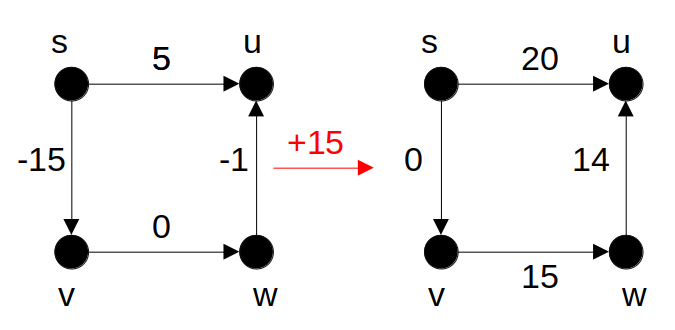
\includegraphics[width=0.4\textwidth]{data/graf_rownowazny_kontrprzyklad.png}
	\caption{  }
	\label{fig:kontrprzyklad_johnson}
\end{figure}

Konstrukcja grafu równoważnego $(G', \omega')$ 
do grafu wejściowego $(G, \omega)$
w algorytmie Johnsona polega na
dodaniu do $G$ wierzchołka $q$, oraz 
dla każdego wierzchołka $v \in V(G)$ krawędzi
skierowanych $qv$ z wagą 0. 

W następnym kroku wywołujemy algorytm Belmmana-Forda
na grafie $(G', w')$ z wierzchołkiem 
startowym $q$ po to, aby utworzyć nową funkcję wagową
na $G$, która zawsze będzie przyjmować wartości 
nieujemne. Umożliwi to zastowanie 
algorytmu Dijsktry. 

\begin{algorithm}[H]
	\caption{Algorytm Johnsona}
	\begin{algorithmic}[1]
		\Procedure{Johnson}{($G, \omega$): graf ważony}
		\State $V' \gets V(G) \cup \{q\}$ 
		\State $E' \gets  E(G) \cup \{qv : v \in V(G)\}$
		\State Skonstruuj graf skierowany $(G', V')$
		\State Zdefiniuj funkcję $w' : E' \to \mathbb{R}$, 
		gdzie 
		\[w'(e) = \begin{cases}
			w(e), &\text{ jeśli } e \in E(G) \\
			0, &\text{ jeśli }  e \not \in E(G)   
		\end{cases}\]
		\State $h \gets \textsc{BellmanFord}((G', w'), q)$
		\State Zdefiniuj funkcję $w'' : E(G) \to \mathbb{R}$, 
		gdzie 
		\[w''(uv) = w(uv) + h(u) - h(v)\]
		\For{$u \in V(G)$}
		\State $d_u = \textsc{Dijsktra}((G, w''), u)$
		\For{$v \in V$}
		\State \textit{odległości}$[u, v] \gets d_u[v] - h[u] + h[v]$
		\EndFor
		\EndFor
		\State \Return \textit{odległości}
		\EndProcedure
	\end{algorithmic}
	\label{Johnson}
\end{algorithm}

Zakładając, że kolejka priorytetowa zastosowana 
w algorytmie Dijsktry jest oparta na kopcach 
Fibonacciego, otrzymujemy złożoność $O(n^2\log n + nm)$. Algorytm 
ten jest szybszy dla grafów rzadkich niż kolejno omawiany 
algorytm Floyda-Warshalla. 

\begin{theorem}[Poprawność algorytmu Johnsona]
	Jeśli $(G, w)$ jest ważonym grafem skierowanym
	bez ujemnych cykli, to algorytm Johnsona dla 
	danych wejściowych $(G, w)$ poprawnie
	rozwiązuje problem najkrótszej ścieżki 
	pomiędzy dowolnymi parami wierzchołków.
	
	\begin{proof}
		Przez $dist_\chi(u, v)$ oznaczmy wagę minimalnej ścieżki
		z wierzchołka $u$ do $v$ przy ważeniu $\chi$ domyślając się, 
		że chodzi o graf $G$ lub $G'$ w zależności od dziedziny $\chi$.
		
		Aby wykazać poprawność aglorytmu Johnsona, 
		musimy udowodnić poniższe obserwacje:
		\begin{enumerate}
			\item Dane wejściowe do 
			algorytmu Bellmana-Forda są poprawne.
			\item Dane wejściowe do 
			algorytmu Dijkstry są poprawne.
			\item Niech $P$ będzie dowolną
			$u$-$v$-ścieżką w grafie $G$ oraz niech $h$
			będzie odwzorowaniem zwróconym przez algorytm
			Belmmana-Forda w linii nr 6. Wtedy
			\[w''(P) = w(P) +  h(u) - h(v).\]
			\item Niech $u, v \in V(G)$, wtedy
			\[dist_{w}(u, v) = dist_{w''}(u, v) - h(u) + h(v).\]
		\end{enumerate}
		
		\paragraph{Dowód obserwacji 1.} Graf ($G$, $w$)
		z założenia nie posiada ujemnych cykli. Ponadto
		dodanie do $G$ wierzchołka $q$ oraz krawędzi skierowanymi
		od $q$ do każdego wierzchołka z $G$ nie może utworzyć
		żadnego nowego cyklu, a więc w szczególności nie może
		w ten sposób powstać żaden ujemny cykl. Oznacza to, że
		$(G', w')$ oraz $q$ to poprawne dane wejściowe
		do algorytmu Bellmana-Forda.
		
		\paragraph{Dowód obserwacji 2.} Niech $uv \in E(G')$. Wtedy prawdą jest, że
		\[dist_{w'}(q, v) \leq dist_{w'}(q, u) + w'(uv),\]
		co w połączeniu z poprawnością algorytmu Belmmana-Forda (tw.
		\ref{bellmanford_proof}) oraz faktem, że 
		$uv \in E(G)$ daje nam
		\[h(v) \leq h(u) + w(uv).\]
		Po przeniesieniu $h(v)$ na prawą stronę otrzymujemy 
		\[0 \leq w(uv) + h(u) - h(v) = w''(uv),\]
		więc każda krawędź grafu ważonego $(G, w'')$ ma
		nieujemną wagę. Wnioskujemy, że wywołanie algorytmu 
		Dijkstry jest poprawne.  
		
		\paragraph{Dowód obserwacji 3.} Niech $P=v_1v_2\dots v_k$, 
		gdzie $v_1 = u$ oraz $v_k = v$ będzie dowolną $u$-$v$-ścieżką
		w grafie $G$. Wtedy 
		\[w''(P) = w''(v_1v_2) + w''(v_2v_3) + \dots + w''(v_{k-1}v_k).\]
		Korzystając z definicji $w''$ otrzymamy
		\[w''(P) = w(v_1v_2) + h(v_1) - (h_2) + 
		w(v_2v_3) + h(v_2) - (h_3) + 
		\dots + w(v_{k-1}v_k) + h(v_{k-1}) - (h_k).\]
		Po uporządkowaniu powyższego dostaniemy
		\[w''(P) = w(P) + w(v_1) - w(v_k) = w(P) + h(u) - h(v),\]
		co należało dowieść.
		
		\paragraph{Dowód obserwacji 4.} Niech $P_{w}$ oraz 
		$P_{w''}$ będą najkrótszymi $u$-$v$-ścieżkami odpowiednio 
		przy ważeniu $w$ oraz $w''$. Korzystając z 
		Obserwacji 3 otrzymujemy
		\[w''(P_{w}) = w(P_{w}) + h(u) - h(v) \leq
		w(P_{w''}) + h(u) - h(v) = w''(P_{w''}),\]
		co wynika, z założenia, że $P_{w}$ to 
		najmniejsza ścieżka w $(G, w)$. 
		
		Z powyższej nierówności oraz z założenia, że $P_{w''}$ to 
		najmniejsza ścieżka w $(G, w'')$ otrzymujemy
		\[w''(P_{w''}) \leq w''(P_{w}) \leq w''(P_{w''}), \]
		\[w''(P_{w''}) = w''(P_{w}).\]
		Po ponownym zastosowaniu obserwacji 3
		\[w''(P_{w''}) = w(P_{w}) + h(u) - h(v),\]
		\[w(P_{w''}) = w''(P_{w''}) - h(u) + h(v).\]
		Dzięki poprawności algorytmu Dijkstry (tw. \ref{dijkstra_proof})
		mamy
		\[dist_{w}(u, v) = dist_{w''}(u, v) - h(u) + h(v).\]
		
		Obserwacje 1, 2 i 4 implikują, że tablica \textit{odległości} zostanie
		wypełniona poprawnie. Jako że algorytm na pewno zakończy pracę,
		dowód poprawności jest kompletny.
	\end{proof} 
\end{theorem}

\subsubsection{Algorytm Floyda-Warshalla}
\begin{algorithm}[H]
	\caption{Algorytm Floyda-Warshalla}
	\begin{algorithmic}[1]
		\Procedure{FloydWarshall}{($G, w$): graf ważony}
		\State Utwórz tablicę odległości o wymiarach $V(G) \times V(G)$
		\For{$i \in V(G)$}
		\For{$j \in V(G)$}
		\If{$ij \in E(G)$}
		\State $\textit{odległości}[i, j] \gets w(ij)$
		\Else
		\State $\textit{odległości}[i, j] \gets \infty$
		\EndIf
		\EndFor
		\EndFor
		\For{$i \in V(G)$}
		\State $\text{odległości}[i, i] \gets 0$
		\EndFor
		\For{$k \in V(G)$}
		\For{$i \in V(G)$}
		\For{$j \in V(G)$}
		\If{$\textit{odległości}[i, j] > \textit{odległości}[i, k] + \textit{odległości}[k, j]$}
		\State $\textit{odległości}[i, j] \gets \textit{odległości}[i, k] + \textit{odległości}[k, j]$
		\EndIf
		\EndFor
		\EndFor
		\EndFor
		\State \Return \textit{odległości}
		\EndProcedure
	\end{algorithmic}
	\label{floydWarshall_alg}
\end{algorithm}

Złożoność powyższego algorytmu to $O(n^3)$.

\begin{theorem}[Poprawność algorytmu Floyda-Warshalla]
	Jeśli $(G, w)$ jest ważonym grafem skierowanym
	bez ujemnych cykli, to algorytm Floyda-Warshalla dla 
	danych wejściowych $(G, w)$ poprawnie
	rozwiązuje problem najkrótszej ścieżki 
	pomiędzy dowolnymi parami wierzchołków.
	
	\begin{proof}
		Oznaczmy przez $d^{(m)}$(i, j) długość najkrótszej
		$i$-$j$-ścieżki, której wewnętrzne wierzchołki 
		należą do zbioru $\{0, 1, 2, \dots, m-1\}$. 
		Ponadto przez
		$\textit{odległości}_{m}[i, j]$ będziemy rozumieli 
		stan tablicy po 
		wykonaniu się $m$-tej iteracji.
		
		\paragraph{Niezmiennik.} Po $l$ iteracjach 
		pętli \textit{for} w linii nr 11, dla każdych wierzchołków
		$i, j \in V(G)$ zachodzi \textit{odległości}$[i,j] \leq d^{(l)}(i,j)$.
		
		\paragraph{Dowód niezmiennika.} Indukcja po liczbie iteracji $l$.
		
		Wartości początkowe spełniają warunek, zatem
		baza indukcyjna jest prawdziwa. 
		
		Przypuśćmy, że $\text{odległości}_{l}[i, j] \leq
		d^{(l)}(i, j)$. Chcemy pokazać, że 
		$\textit{odległości}_{l+1}[i, j] \leq$$ d^{(l+1)}(i, j)$.
		W przypadku, kiedy $d^{(l)}(i,j) =$$ d^{(l+1)}(i,j)$, to
		\[d^{(l+1)}(i,j) = d^{(l)}(i, j) \geq 
		\text{odległości}_l[i, j] \geq \text{odległości}_{l+1}[i, j],\]
		gdzie pierwsza nierówność wynika z założenia indukcyjnego, natomiast
		druga z 14 i 15 linii algorytmu, które implikują, że
		w każdej iteracji wartości w tablicy \textit{odległości} mogą jedynie się zmniejszyć lub
		nie ulec żadnej zmianie.
		
		Rozważmy przypadek kiedy $d^{(l)}(i,j) >$$ d^{(l+1)}(i,j)$. 
		W takiej sytuacji musiała powstać co najmniej jedna 
		$i$-$j$-ścieżka. Każda z nowopowstałych $i$-$j$-ścieżek
		musi zawierać w sobie wierzchołek $l$. Niech 
		$P$ będzie najkrótszą z nich. Zauważmy, że
		\[w(P) = d^{(l+1)}(i, j) = 
		d^{(l+1)}(i, l) + d^{(l+1)}(l, j),\]
		gdzie druga równość wynika z wielokrotnego zastosowania 
		lematu \ref{minpath_subpath}.
		
		Ponadto możemy zauważyć, że $d^{(l+1)}(i, l) = d^{(l)}(i, l)$ 
		oraz $d^{(l+1)}(l, j) = d^{(l)}(l, j)$. Wynika to z faktu, że
		najkrótsza ścieżka zaczynająca się w $l$, której wnętrze składa się z wierzchołków 
		$\{0, 1, 2, \dots, l-1\}$,
		nie może być gorsza niż najkrótsza ścieżka, której 
		wnętrze składa się z wierzchołków 
		$\{0, 1, 2, \dots, l-1, l\}$.
		
		Zatem ostatecznie:
		\begin{gather*}
		\text{odległości}_{l+1}[i,j] \leq 
		\text{odległości}_{l}[i,l] + \text{odległości}_{l}[l,j] \leq
		\\
		\leq d^{(l)}(i, l) + d^{(l)}(l, j) = d^{(l+1)}(i, l) + d^{(l+1)}(l, j) = d^{(l+1)}(i, j),
		\end{gather*}
		gdzie pierwsza nierówność wynika z 14 oraz 15 linii algorytmu,
		natomiast druga -- z założenia indukcyjnego.
		
		Na mocy indukcji matematycznej niezmiennik jest prawdziwy.
		
		\paragraph{Stwierdzenie. } W każdym momencie działania algorytmu
		dla każdego wierzchołka $v \in V(G)$ zachodzi 
		\[\textit{odległość}[v] \geq d(v).\]
		
		\paragraph{Dowód stwierdzenia.} Indukcja po liczbie iteracji $l$.
		
		Dla zerowej liczby wywołań teza jest spełniona, a 
		zatem baza indukcyjna jest prawdziwa.
		
		Przyjmijmy, że jeśli $\textit{odległości}_l[i, j] \geq d(i, j)$
		jest prawdą, to $\textit{odległości}_{l+1}[i, j] \geq d(i, j)$
		również musi być prawdziwe.
		
		Jeśli $\textit{odległość}_{l+1}[i, j] = \textit{odległość}_{l}[i, j]$,
		to korzystając z założenia indukcyjnego, możemy zakończyć dowód.
		
		Rozważmy przypadek, kiedy 
		$\textit{odległość}_{l+1}[i, j] < \textit{odległość}_{l}[i, j]$. 
		Aby ten przypadek zaszedł, musiały wykonać się linijki 14 i 15.
		Oznacza to, że 
		\[\textit{odległość}_{l+1}[i, j] = \textit{odległość}_{l}[i, l+1] 
		+ \textit{odległość}_{l}[l+1, j] \geq d(i, l+1) + d(l+1, j)
		\geq d(i, j),\]
		gdzie pierwsza nierówność wynika z założenia indukcyjnego,
		natomiast druga z faktu, że $d(i, j)$ oznacza
		długość najkrótszej ścieżki.
		
		Na mocy indukcji matematycznej stwierdzenie jest prawdziwe.
		
		Stwierdzenie oraz niezmiennik implikują, że 
		dla każdej pary wierzchołków
		$i, j \in V(G)$ prawdą jest, że 
		\[\textit{odległość}_n[i,j] \leq d^{(n)}(i, j) = d(i, j) \leq \textit{odległość}_n[i,j],\]
		a zatem
		\[\textit{odległość}_n[i,j] = d(i, j),\]
		co kończy dowód. \qedhere
	\end{proof} 
	\label{floydWarshall_proof}
\end{theorem}

\subsubsection{Podsumowanie}
\section{Problem najkrótszej ścieżki -- Zadania}
\subsection{Zadanie 1 -- Algorytm Bellmana-Forda z odtwarzaniem ścieżki}
\paragraph{Treść.}Zmodyfikuj algorytm Bellmana-Forda tak, 
aby znajdował najkrótszą ścieżkę między zadanymi dwoma
wierzchołkami.

\paragraph{Rozwiązanie.}

\begin{algorithm}[H]
	\caption{Algorytm Bellmana-Forda z odtwarzaniem ścieżki}
	\begin{algorithmic}[1]
		\Procedure{BellmanFord}{$(G, w)$: graf ważony, $s$: wierzchołek startowy, $t$: wierzchołek docelowy}

		\State odległość = tablica liczb, rozmiaru $V[G]$
		\State poprzednik = tablica wierzchołków, rozmiaru $V[G]$
		\For{$v \in V(G)$}
		\State odległość$[v]\gets\infty$
		\State poprzednik$[v]\gets-1$
		\EndFor
		\State odległość$[s]\gets0$
		\For{$i=1,2,\dots,n-1$}
		\For{$uv \in E(G)$}
		\If{odległość$[v] >$ odległość$[u]$ + $w(uv)$}
		\State odległość$[v]\gets$ odległość$[u] + w(uv)$ 
		\State poprzednik$[v]\gets u$
		\EndIf
		\EndFor
		\EndFor
		\State ścieżka $\gets$ pusta lista wierzchołków
		\State ściezka.PushFront($t$)
		\While{$t \gets \text{poprzednik}[t] \not = -1$}
		\State ścieżka.PushFront($t$)
		\EndWhile
		\State \Return ścieżka
		\EndProcedure
	\end{algorithmic}
	\label{Zadanie31}
\end{algorithm}
\subsection{Zadanie 2 -- Szukanie ujemnego cyklu}
\paragraph{Treść.}Zaprojektuj algorytm, który znajdzie w 
ważonym grafie skierowanym ujemny cykl, jeśli taki istnieje.
Wskazówka: zmodyfikuj algorytm Bellmana-Forda.

\paragraph{Rozwiązanie.}
Rozwiązanie polega na sprawdzeniu, czy wykonanie
jeszcze jednej nadmiarowej iteracji 
w algorytmie Bellmana-Forda %robi co??
, oraz sprawdzenie
czy pewien wierzchołek został poprawiony. % ale co z tym sprawdzeniem?

Jeżeli poniższy warunek jest spełniony
\[\exists_{v\in V(G)}\quad \text{odległość}_n[v] < \text{odległość}_{n-1}[v],\]
to w grafie $G$ musi istnieć ujemny cykl. Dzieje się 
tak, ponieważ zawsze istnieje co najmniej jedna krawędź 
w cyklu ujemnym $C$, która spełnia warunek 
\[\text{odległość}[v] > \text{odległość}[u] + w(uv),\]
zatem będzie wtedy istniał wierzchołek, który zostanie 
poprawiony.

Jako że graf wejściowy może być niespójny,
musimy dodać dodatkowy wierzchołek $s$, który
będzie połączony z każdym innym wierzchołkiem
przy pomocy krawędzi skierowanej od wierzchołka $s$. Jako
że żadna krawędź nie wchodzi do wierzchołka $s$, możemy mieć pewność,
że żadne nowe cykle nie powstaną. Zatem
w szczególności nie powstaną nowe
ujemne cykle.

\begin{algorithm}[H]
	\caption{Znajdowanie ujemnego cyklu}
	\begin{algorithmic}[1]
		\Procedure{BellmanFord}{($G, w$): graf ważony}
		\State $G'$ $\gets$ graf $G$ z dodanym wierzchołkiem $s$
		oraz krawędziami skierowanymi od $s$ do każdego innego
		wierzchołka o wadze $0$
		\State odległość $\gets$ tablica liczb, rozmiaru $V[G']$
		\For{$v \in V(G')$}
		\State odległość$[v]\gets\infty$
		\EndFor
		\State odległość$[s]\gets0$
		\For{$i=1,2,\dots,n-1$}
		\For{$uv \in E(G')$}
		\If{odległość$[v] >$ odległość$[u]$ + $w(uv)$}
		\State odległość$[v]\gets$ odległość$[u] + w(uv)$ 
		\EndIf
		\EndFor
		\EndFor
		\For{$uv \in E(G')$}
		\If{odległość$[v] >$ odległość$[u]$ + $w(uv)$}
		\State return \true
		\EndIf
		\EndFor
		\State \Return \false
		\EndProcedure
	\end{algorithmic}
	\label{Zadanie32}
\end{algorithm}

\subsection{Zadanie 3 -- Szukanie liczby spacerów o zadanej liczbie krawędzi}
\paragraph{Treść.}
Zaprojektuj algorytm, który dla danego grafu prostego 
$G$, wierzchołków $u, v \in V(G)$ i liczby $k \in
\{1, 2, \ldots , n\}$ znajdzie liczbę spacerów 
od $u$ do $v$ o dokładnie $k$ krawędziach.

%\paragraph{Rozwiązanie.}% :(

\subsection{Zadanie 4 -- Wyznaczanie odległości w drzewie ważonym}
\paragraph{Treść.}Zaprojektuj algorytm, który dla ważonego 
acyklicznego grafu skierowanego $G$ oraz wierzchołków $s, t \in
V(G)$ wyznaczy odległość od $s$ do $t$ w czasie $O(m)$. 
Wskazówka: wykorzystaj sortowanie topologiczne (zadanie \ref{zad:tsort}).

\paragraph{Rozwiązanie.}
Dijkstra tylko, że zamiast kolejki $Q$ stosujemy
sortowanie topologiczne (średnia złożoność $O(m)$), 
po czym iter % PO CZYM ITER CO? :( po czym iter co...
\begin{algorithm}[H]
	\caption{Znajdowanie ujemnego cyklu}
	\begin{algorithmic}[1]
		\Procedure{FindDistanceInTree}{($T, w$): drzewo ważone}
		\State Niech odległość to tablica liczb, rozmiaru $V[G]$
		\State Niech kolejność to tablica liczb, rozmiaru $V[G]$, na
		$i$-tej komórce znajduje się wierzchołek, który ma 
		$i$-te miejsce w posortowanej topologicznie tablicy wierzchołków
		\State kolejność $\gets$ \textsc{TSort}($T$)
		\For{$i = 0, 1, \dots n - 1$}
		\State $u \gets \text{kolejność}[i]$
		\For{$v \in N(u)$}
		\If {$\text{odległość}[u] + w(uv) < 
			\text{odległość}[v]$}
		\State $\text{odległość}[v] \gets \text{odległość}[u] + w(uv)$
		\EndIf
		\EndFor 
		\EndFor
		\State \Return \false
		\EndProcedure
	\end{algorithmic}
	\label{Zadanie34}
\end{algorithm}

\subsection{Zadanie 5 -- Naiwna wersja algorytmu A\texorpdfstring{$^*$}{TEXT}}
\paragraph{Treść.}Znajdź przykład, dla 
którego algorytm A$^*$ nie zadziała zgodnie z oczekiwaniami, 
w którym spełnione
są wszystkie założenia 
poza 
,,dla każdej krawędzi $uv$ zachodzi $h(u) \leq h(v) + w(uv)$''.

\paragraph{Rozwiązanie.}% :/

\subsection{Zadanie 6 -- Poprawność algorytmu A\texorpdfstring{$^*$}{TEXT}}
\paragraph{Treść.}Udowodnij poprawność algorytmu 
A$^*$ i wskaż, w których miejscach wykorzystywane są jego założenia.
Wskazówka: zainspiruj się dowodem poprawności algorytmu Dijkstry.

\paragraph{Rozwiązanie.}Dowód twierdzenia \ref{aStar_proof}.

\subsection{Zadanie 7 -- Poprawność algorytmu Floyda-Warshalla}
\paragraph{Treść.}Udowodnij poprawność algorytmu Floyda-Warshalla. 
Wskazówka: niech 
$d^{(m)}(i, j)$ będzie długością
najkrótszej ścieżki od $i$ do $j$, której wewnętrzne wierzchołki należą
do zbioru $\{0, 1, 2, . . . , m - 1\}$; 
udowodnij, że po $l$
iteracjach zewnętrznej pętli dla każdych $i, j \in V (G)$ zachodzi 
odległość$[i, j] \leq d^{(l)}(i, j)$.

\paragraph{Rozwiązanie.}Dowód twierdzenia \ref{floydWarshall_proof}.

\section{Przepływy}
\subsection{Wstęp}
\begin{defi}
	Sieć przepływowa to graf skierowany $G$
	z funkcją wag $c: E(G) \to 
	\mathbb{R}_{\geq 0} \cup \{\infty\}$ oraz
	wyróżnionymi wierzchołkami $s$ i $t$. Mówimy, że
	\begin{itemize}[noitemsep, nolistsep]
		\item $c(e)$ to przepustowość krawędzi $e \in E(G)$,
		\item $s$ to źródło (ang. source),
		\item $t$ to ujście (ang. target).
	\end{itemize}
\end{defi}

\begin{defi}
	Przepływem nazywamy funkcję $f: E(G) \to \mathbb{R}_{\geq 0}$ 
	taką, że 
	\begin{itemize}
		\item $f(e) \leq c(e)$ dla każdej krawędzi $e\in E(G)$,
		\item $f^+(v) = f^-(v)$ dla każdego wierzchołka $v \in V(G) \setminus \{s, t\}$,
	\end{itemize}
	gdzie $f^+(v) := \sum\limits_{u:vu \in E(G)} f(vu)$ oraz $f^-(v) := \sum\limits_{u:uv \in E(G)} f(uv)$,
	tak samo jeśli $S \subset V(G)$, to $f^+(S) := \sum\limits_{uv \in E(G), u\in S \land v \not \in S  } f(uv)$ oraz 
	$f^-(S) := \sum\limits_{uv \in E(G), u\not \in S \land v \in S  } f(uv)$
\end{defi}

\begin{defi}
	Wartością przepływu nazywamy różnicę 
	$\val(f)=f^+(s)-f^-(s)$.
\end{defi}

\subsection{Problem maksymalnego przepływu}
Dana jest sieć przepływowa $(G, c, s, t)$ szukamy przepływu $f$
o maksymalnej możliwej wartości $\text{val}(f)$. 

\begin{defi}
	Sieć rezydualna dla danej sieci przepływowej $(G, c, s, t)$
	oraz przepływu $f$ to graf skierowany $R$ o zbiorze
	wierzchołków $V(G)$, funkcji $c_f$ oraz zbiorze krawędzi
	równym $\{uv : c_f(uv) > 0\}$, gdzie funkcja $c_f$ jest 
	zdefiniowana następująco
	\begin{itemize}
		\item $c_f(uw) = c(uw) - f(uw)$, gdy $uw \in E(G)$ oraz $wu \not \in E(G)$ (krawędź w przód)
		\item $c_f(uw) = f(wu)$, gdy $uw \not \in E(G)$ oraz $wu \in E(G)$ (krawędź wstecz)
		\item $c_f(uw) = c(uw) - f(uw) + f(wu)$, gdy 
		$uw \in E(G)$ oraz $wu \in E(G)$
	\end{itemize}
\end{defi}

Intuicyjnie $c_f(uw)$ możemy
rozumieć jako określenie ile jednostek przepływu 
jesteśmy w stanie ,,przepuścić'' z $u$ do $w$, co
możemy osiągnąć, albo zwiększając przepływ na krawędzi $uw$
albo zmniejszając przepływ na krawędzi $wu$.

Warto zauważyć, że w sieci rezydualnej rozpatrujemy tylko te 
krawędzie, dla których przepustowość rezydualna jest większa niż 0.

\begin{defi}
	Ścieżką powiększającą nazywamy dowolną ściężką od $s$
	do $t$ w sieci rezydualnej. 
\end{defi}

Zauważmy, że jeśli znajdziemy ścieżkę powiększającą $P$ 
w sieci rezydualnej,
to wartość przepływu $f$ jesteśmy w stanie powiększyć o 
$\min\limits_{uw \in E(P)} \{c_f(uw)\}$.

\subsubsection{Algorytm Forda-Fulkersona}

\begin{algorithm}[H]
	\caption{Algorytm Forda-Fulkersona}\label{ford-fulker_alg}
	\begin{algorithmic}[1]
		\Procedure{FordFulkerson($(G, w)$, $s$, $t$)}{}
		\State Niech $f$ to zerowy przepływ w sieci $(G,c,s,t)$
		\State Utwórz sieć rezydualną $(R, c_f)$ dla wejściowej 
		sieci przepływowej oraz dla $f$ 
		\While{Istnieje ścieżka powiększająca $P$ w $R$}
		\State Oznaczmy $P = v_1v_2\dots v_k$ (gdzie $v_1 = s$ oraz $v_k = t$)
		\State $a \gets \min_{i \in \{1, 2, \dots, k-1\}} r(v_iv_{i+1})$
		\State Powiększ $f$ o $a$ na wszystkich krawędziach $P$
		\State Uaktualnij $(R, c_f)$ na wszystkich krawędziach $P$
		\EndWhile
		\State \Return $f$
		\EndProcedure
	\end{algorithmic}
\end{algorithm}

\begin{theorem}
	[Twierdzenie Forda-Fulkersona] Przepływ ma maksymalną wartość wtedy i tylko 
	wtedy, gdy nie istnieje ścieżka powiększająca.
	\begin{proof}
		MD2
	\end{proof}
\end{theorem}

Uwaga: zwykle 
zakładamy, że przepustowości krawędzi są liczbami całkowitymi, 
ponieważ, wówczas po każdym 
wykonaniu pętli while, wartość przepływu $f$ zwiększy się
przynajmniej o 1, co umożliwia oszacowanie
złożoności algorytmu. 

Możemy oszacować, że algorytm Forda-Flukersona 
zakończy się w czasie $O(mf_{\max})$, gdzie 
przez $f_{\max}$ oznaczamy wartość maksymalnego przepływu. 
Z tego oszacowania wnioskujemy, że dla sieci, w których
maksymalna wartość przepływu jest duża, 
nie warto stosować tego algorytmu. 

\subsubsection{Algorytm Edmondsa-Karpa}
Algorytm Edmondsa-Karpa różni się od 
algorytmu Forda-Fulkersona tylko tym, że
w pętli while operujemy na najkrótszej ścieżce powiększającej
zamiast na dowolnej.

Taka modyfikacja daje nam gwarancję, że
algorytm zakończy się w czasie wielomianowym.

\begin{algorithm}[H]
	\caption{Edmonds-Karp}\label{edmonds-karp_alg}
	\begin{algorithmic}[1]
		\Procedure{EdmondsKarp($G, w$, $s$, $t$))}{}
		\State Niech $f$ to zerowy przepływ w sieci $(G,c,s,t)$
		\State Utwórz sieć rezydualną $(R, c_f)$ dla wejściowej 
		sieci przepływowej oraz dla $f$ 
		\While{Istnieje ścieżka powiększająca w $R$}
		\State Niech $P = v_1v_2\dots v_k$ będzie \textbf{najkrótszą}
		ścieżką powiększająca (gdzie $v_1 = s$ oraz $v_k = t$)
		\State $a \gets \min_{i \in \{1, 2, \dots, k-1\}} r(v_iv_{i+1})$
		\State Powiększ $f$ o $a$ na wszystkich krawędziach $P$
		\State Uaktualnij $(R, c_f)$ na wszystkich krawędziach $P$
		\EndWhile
		\State \Return $f$
		\EndProcedure
	\end{algorithmic}
\end{algorithm}


\begin{theorem}
	Algorytm Edmondsa-Karpa dla zadanej sieci przepływowej $(G, c, s, t)$
	zakończy się w czasie $O(nm^2)$, gdzie $n$ i $m$ to dopowiednio
	liczba wierzchołków i liczba krawędzi grafu skierowanego $G$.
	\begin{proof}
		Dla dowolnego przepływu $f$ w sieci $(G, c, s, t)$ i wierzchołków
		$u, v \in V(G)$ przez $d_f(u, v)$, będziemy oznaczali najmniejszą
		możliwą liczbę krawędzi na $u$-$v$-ścieżce w sieci 
		rezydualnej odpowiadającej przepływowi $f$ (inaczej: odległość
		od $u$ do $v$ w sensie liczby krawędzi w sieci rezydualnej dla $f$).
		
		Niech $P_1, P_2, \dots P_k$ to wszystkie najkrótsze
		$s$-$v$-ścieżki w sieci rezydualnej odpowiadającej przepływowi
		$f$, wtedy 
		\[L_f := \left|\bigcup_{i \in [k]} E(P_i)\right|.\]
		
		\textbf{Stwierdzenie 1:} Niech $f$ będzie przepływem przed
		pewną iteracją pętli w linii nr. 4, a $f'$ przepływem 
		po tej iteracji. Wówczas
		dla każdego $v$ zachodzi $d_{f'}(s, v) \geq d_{f}(s,v)$,
		
		\textbf{Dowód stwierdzenia 1:}
		Przypuśćmy, że tak nie jest, tzn., że istnieje 
		taki wierzchołek $v \in V(G)$, że $d_{f'}(s, v) < d_f(s,v)$.
		Bez straty ogólności przyjmijmy, że $v$
		minimalizuje $d_{f'}(s,v)$ spośród takich problematycznych 
		wierzchołków - tzn., że dla każdego wierzchołka $x$, dla 
		którego $d_{f'}(s, x) < d_{f'}(s, v)$ prawdą jest, że 
		$d_{f'}(s, x) \geq d_f(s,x)$.
		
		Niech $P'$ to najkrótsza w sensie liczby krawędzi $s$-$v$-ścieżka
		w sieci rezydualnej odpowiadającej $f'$. Przez $w$ oznaczmy 
		przedostatni wierzchołek na ścieżce $P'$. Rozpatrzmy
		teraz dwa przypadki:
		\begin{itemize}
			\item[1.] Krawędź $wv$ należy do sieci rezydualnej 
			odpowiadającej
			przepływowi $f$, tzn. $c_f(wv) > 0$. W takiej 
			sytuacji możemy zapisać, że  
			\[d_f(s, v) \leq d_f(s, w) + 1 \leq d_{f'}(s, w) + 1 = d_{f'}(s, v),\]
			gdzie pierwsza nierówność wynika z faktu, że sieć rezydualna $f$
			ma krawędź od $w$ do $v$, druga z minimalności $v$ (tzn. 
			$w$ znajduje się bliżej źródła niż $v$), a ostatnia równość
			wynika stąd, że $w$ poprzeda $v$ na najkrótszej ścieżce 
			w sieci rezydualnej dla $f'$ (z doboru $P'$).
			Powyższy ciąg nierówności stoi w sprzeczności z
			$d_{f'}(s, v) < d_f(s,v)$.
			
			\item[2.] Krawędź $wv$ nie należy do sieci rezydualnej 
			odpowiadającej
			przepływowi $f$, tzn. $c_f(wv) = 0 \implies c(wv) = f(wv)$.
			Skoro  $c_{f'}(wv) > 0$, to oznacza, że przepływ na
			krawędzi $wv$ podczas wykonywania się iteracji zmienił się, 
			co w połączeniu z faktem, że  $c_f(wv) = 0$
			implikuje, że krawędź $vw$ musiała być częścią ścieżki 
			powiększającej wybranej w linii nr 5 w tej iteracji.
			Zatem 
			\[d_f(s, w) = d_f(s, v) + 1,\]
			co doprowadza nas do 
			\[d_f(s, v) = d_f(s,w) - 1 \leq
			d_{f'}(s,w) -1 = d_{f'}(s,v    ) - 2 < d_{f'}(s,v)\]
			Powyższy ciąg nierówności stoi w sprzeczności z
			$d_{f'}(s, v) < d_f(s,v)$.
		\end{itemize}
		
		Zatem stwierdzenie 1 jest prawdziwe.
		
		\textbf{Stwierdzenie 2:} Niech $f$ będzie przepływem przed
		pewną iteracją pętli w linii nr. 4, a $f'$ przepływem 
		po tej iteracji. Wówczas 
		jeżeli $d_{f'}(s, t) = d_f(s,t)$, to $L_{f'} < L_f$.
		
		\textbf{Dowód stwierdzenia 2:} Najpierw pokażemy, że
		każda krawędź licząca się do $L_{f'}$, musi zaliczać się
		również do $L_f$. W tym celu rozważmy pewną najkrótszą (względem
		liczby krawędzi) ścieżkę $P' = w_0 w_1 \dots w_k$,
		w sieci rezydualnej dla $f'$,
		gdzie $s = w_0$, $t = w_k$ oraz $k = d_{f'}(s, t)$.
		Rozważmy odległości kolejnych wierzchołków na ścieżce 
		od $s$ w sieci rezydualnej dla $f$. 
		
		Rozważmy dwa przypadki dla krawędzi $w_i w_{i+1}$:
		\begin{itemize}
			\item[1.] Krawędź $w_i w_{i+1}$ była obecna w sieci rezydualnej
			dla przepływu $f$, wtedy musi zachodzić 
			\[d_f(w_{i+1}) \leq d_f(w_{i}) + 1.\]
			\item[2.] Krawędź $w_i w_{i+1}$ nie była obecna w sieci rezydualnej
			dla przepływu $f$, wtedy musi zachodzić
			\[d_f(w_{i+1}) \leq d_f(w_{i}) - 1,\]
			ponieważ krawędź $w_i w_{i+1}$ została dodana
			do sieci rezydualnej $f'$ wskutek powiększenia przepływu
			wzdłuż ścieżki $P$ wybranej w linii nr. 5.
		\end{itemize}
		
		Kumulując powyższe przypadki, otrzymamy
		\[d_{f}(s, t) \leq d_{f}(s, w_{k-1}) \pm 1 \leq
		(d_{f}(s, w_{k-2}) \pm 1) \pm 1 \leq \ldots \leq A - B,\]
		gdzie $A$ oznacza liczbę wystąpień przypadku 1., z kolei
		$B$ - liczbę wystąpień przypadku 2. Ale z założenia 
		$d_{f'}(s,t)=d_f(s,t)$, więc ścieżka $P'$ ma dokładnie $d_f(s,t)$
		krawędzi, co pociąga za sobą $B = 0$ (bo wyrażenie
		$A-B$ jest maksymalnie równe $d_f(s,t)$), z czego wynika, 
		że żadna z krawędzi 
		ścieżki $P'$ nie może realizować przypadku 2. Z tego 
		rozumowania wynika, że każda krawędź na ścieżce $P'$
		znajdowała się w sieci rezydualnej dla $f$. Z dowolności wyboru
		$P'$ każda krawędź licząca się do $L_{f}$ musi też zaliczać się
		do $L_{f'}$, co chcieliśmy pokazać.
		
		Teraz zauważmy, że przynajmniej jedna krawędź wliczająca
		się do $L_f$ nie wlicza się do $L_{f'}$, jest to krawędź 
		o przepustowości $a$ (linijka nr. 6), która znajduje się
		na ścieżce $P$ wybranej w linii nr. 5. Zatem ostatecznie 
		\[L_{f'} < L_f,\]
		a więc dowód stwierdzenia 2. jest kompletny.
		
		Z obu powyższych stwierdzeń możemy wywnioskować, dwa przypadki
		\begin{itemize}
			\item[1.] $d_{f'}(s, t) > d_f(s, t)$,
			\item[2.] $d_{f'}(s, t) = d_f(s, t) \Rightarrow 
			L_{f'} < L_f$.
		\end{itemize}
		Oba powyższe przypadki implikują, że z sieci rezydualnej została 
		usunięta co najmniej jedna krawędź, co pozwala nam 
		dokonać oszacowania.
		
		W pesymistycznym przypadku mamy $n-1$ $s$-$t$-ścieżek oraz 
		pesymistycznie usuwamy dokładnie jedną krawędź w każdej iteracji
		co ostatecznie daje nam nie więcej niż $nm$ wywołań pętli w nr 4.
		Ponadto w każdej iteracji wywołujemy BFS w celu znalezienia najkrótszej
		ścieżki, z kosztem $O(m)$. Zatem złożoność algorytmu Edmondsa-Karpa
		to $O(nm^2)$. \textbf{TODO Marcin:} \textit{Wytłumaczyć to inaczej}
		
	\end{proof}
\end{theorem}

\subsection{Problem MinCostMaxFlow}
\textbf{Dane:}
\begin{itemize}
	\item Sieć przepływowa $(G, c, s, t)$
	\item Funkcja kosztu $k : E(G) \to \mathbb{R}$
\end{itemize}

\textbf{Szukane:}
Maksymalny przepływ $f$, który minimalizuje koszt 
\[k(f) := \sum_{e\in E(G)}k(e)f(e).\]

Ten problem możemy rozumieć jako wybranie takiego przepływu $f$ 
ze wszystkich maksymalnych przepływów, dla którego
$k(f)$ jest najmniejsze. 

\begin{defi}
	Siecią rezydualną z kosztami dla danej sieci przepływowej
	$(G, c, s, t)$, funkcji kosztów $k$ i przepływu $f$ nazywamy
	graf skierowany $R$ o zbiorze wierzchołków $V(G)$, funkcji
	wag $c_f$, funkcji kosztów $k_f$ oraz zbiorze 
	krawędzi równym $\{ uv: c_f(uv) > 0\}$, gdzie funkcje 
	$c_f$ i $k_f$ są zdefiniowane następująco:
	\begin{itemize}
		\item $c_f(uw) = c(uw) - f(uw)$ i $k_f(uw) = k(uw)$,
		jeśli $uw \in E(G)$ oraz $wu \not \in E(G)$
		\item $c_f(uw) = f(uw)$ i $k_f(uw) = -k(uw)$,
		jeśli $uw \not \in E(G)$ oraz $wu \in E(G)$
	\end{itemize} 
\end{defi}
W powyższej definicji nie uwzględniamy przypadku kiedy 
$uw \in E(G)$ oraz $wu \in E(G)$, ponieważ w takiej sytuacji
sieć rezydualna jest multigrafem, który utrudnia reprezentację. 
Jako, że taką sytuację można łatwo rozwiązać tworząć podpodział
krawędzi $uw$ lub $wu$, przyjmujemy, że operujemy na grafach,
w których takie sytuacje nie występują.

\begin{theorem}
	[Twierdzenie o minimalnym koszcie] Niech $f$ będzie
	maksymalnym przepływem w sieci $(G, c, s, t)$ z funkcją 
	kosztu $k$. Wówczas $f$ jest maksymalnym przepływem 
	o minimalnym koszcie wtedy i tylko wtedy, gdy 
	odpowiadająca mu sieć rezydualna z kosztami
	nie zawiera cyklu o ujemnym koszcie.
	\begin{proof}
		Przez $(R_f, c_f, k_f)$, będziemy oznaczali sieć rezydualną
		z kosztami odpowiadającą przepływowi $f$, gdzie $c_f$ 
		jest funkcją przepustowości, a $k_f$ funkcją kosztów.
		Zauważmy, że $(R_f, c_f)$ oraz $(R_f, k_f)$ są ważonymi 
		grafami skierowanymi.
		
		Najpierw pokażemy, że jeśli $(R_f, k_f)$ zawiera ujemny cykl,
		to maksymalny przepływ $f$ nie minimalnego kosztu.
		Niech $C$ będzie ujemnym cyklem w $(R_f, k_f)$, tzn. $k_f(C) < 0$.
		Niech $a$ to najmniejsza przepustowość w $(R_f, c_f, k_f)$, pewnej
		krawędzi na $C$, tzn.
		\[a := \min_{uw \in C} c_f(uw) > 0,\]
		gdzie nierówność wynika z definicji sieci rezydualnej. Rozważmy 
		przepływ $f'$, taki, że, dla każdego
		$e \in E(G)$
		\[f'(e) = \begin{cases} 
			f(e) + a, &  e \in C \\
			f(e), & e \notin C.
		\end{cases}\]
		Zauważmy, że wartość przepływu $f'$ jest taka sama
		jak wartość przepływu $f$, zatem $f'$ również jest
		maksymalnym przepływem. Ponadto zachodzi 
		\[k(f') = k(f) + ak_f(C),\]
		skoro $k_f(C)$ jest ujemne, to 
		\[k(f') > k(f),\]
		czyli znaleźliśmy inny przepływ maksymalny o mniejszym koszcie
		co kończy tę część dowodu.
		
		Pokażemy teraz, że jeśli maksymalny przepływ $f$
		nie jest minimalnego kosztu, to w $(R_f, k_f)$ musi istnieć
		ujemny cykl. Rozważmy przepływ $f'$, który jest
		maksymalnym przepływem o minimalnym koszcie różniącym
		się od $f$ na najmniejszej możliwej liczbie krawędzi tzn.
		dla każdego maksymalnego przepływu $f''$ prawdą jest, że
		\[|\{e \in E(G) : f'(e) \not = f(e)\}| \leq 
		|\{e \in E(G) : f''(e) \not = f(e)\}|.\]
		Niech $S$ będzie zbiorem krawędzi sieci rezydualnej dla $f$ 
		takich, że przepuszczenie dodatkowego (dodatniego)
		przepływu wzdłuż tych krawędzi przybliży $f$ do $f'$, tzn.
		\[S = \{uw : f(uw) < f'(uw) \lor f(wu) > f'(wu)\}.\]
		Przez $S'$ oznaczmy krawędzie sieci rezydualnej dla $f'$
		odwrotne do $S$.
		
		Zauważmy, że wartości przepływów $f$ i $f'$ są równe (bo oba są
		maksymalnymi przepływami), a więc dla każdego wierzchołka
		$v \in V(G)$ otrzymujemy
		\[f^+(v) - f^-(v) = f^{'+}(v) - f^{'-}(v),\]
		bo dla $v \in \{s, t\}$ otrzymujemy po obu 
		stronach wartość przepływu, która jest taka sama, a
		dla  $v \not \in \{s, t\}$ otrzymujemy zero z definicji przepływu.
		Przekształcając tę równość otrzymujemy
		\[f^{'+}(v) - f^+(v) = f^{'-}(v) - f^{-}(v),\]
		więc jeśli do $v$ wchodzi jakaś krawędź z $S$, to 
		z powyższej równości oraz definicji $S$ wynika, że
		musi z niego wychodzić jakaś krawędź z $S$. Jako, że
		liczba wierzchołków jest skończona powyższy fakt musi 
		pociągać za sobą istnienie cyklu wewnątrz zbioru $S$ (bo
		nie możemy wychodzić
		do nieodwiedzonego wierzchołka w nieskończoność).
		
		Niech $C$ będzie cyklem w $S$, a więc również 
		cyklem w sieci rezydualnej $f$; przez $C'$ oznaczmy
		odwrotność cyklu $C$, tzn. $C' := \{wu : uw \in C\}$.
		Zauważmy, że $C'$ jest cyklem w $S'$, a więc jest
		również cyklem w sieci rezydualnej $f'$. 
		
		Ponadto oznaczmy
		przez $a$ najmniejszą wartość z $f'(uw) - f(uw)$ po krawędziach
		$uw \in C$ spełniających $f(uw) < f'(uw)$ oraz z 
		$f(wu) - f'(wu)$ po krawędziach $wu \in C$ spełniających
		$f(wu) > f'(wu)$. Intuicyjnie, $a$ jest taką wartościa, 
		że
		możemy powiększyć przepływ $f$ wzdłuż cyklu $C$ o $a$ 
		nie przekraczając przepustowości krawędzi oraz 
		takie powiększenie
		spowoduje, że któraś z krawędzi $C$ przestanie 
		„zaliczać się” do zbioru $S$.
		
		Zauważmy, że gdyby $k_f(C) > 0$ , wówczas $k_{f'}(C) < 0$
		co jest sprzeczne, bo $f'$ jest maksymalnym
		przepływem o minimalnym koszcie a już pokazaliśmy,
		że to implikuje brak ujemnych cykli
		w sieci rezydualnej z kosztem.
		
		W przypadku kiedy $k_f(C) = 0$ to oznaczałoby że $k_{f'}(C)=0$,
		a więc przepływ $f'' := f' + aC'$, czyli przepływ otrzymany
		z $f'$ poprzez powiększenie wzdłuż cyklu $C'$ o $a$ również 
		jest maksymalnym przepływem o minimalnym koszcie, jednakże
		ze sposobu wyboru $a$ wynika, że $f''$ różni się od $f$
		na mniejszej liczbie krawędzi niż $f'$, co stoi w 
		sprzeczności ze sposobem wyboru $f'$.
		
		Oznacza to, że $k_f(C) > 0$ co kończy dowód.
		
	\end{proof}
	\label{mincost_maxflow_proof}
\end{theorem}

\begin{algorithm}[H]
	\caption{Algorytm ,,Przez usuwanie cykli''}
	\begin{algorithmic}[1]
		\Procedure{CycleCanceling(($G, c, s, t$), $k$)}{}
		\State $f \gets $ maksymalny przepływ dla $(G,c,s,t)$
		\State $(R,c_f,k_f) \gets $ sieć rezydualna dla $f$
		\While{Istnieje ujemny cykl $C$ w $(R, k_f)$}
		\State $a \gets \min\{c_f(uw) : uw \in C\}$
		\State Powiększ $f$ o $a$ na wszystkich krawędziach $C$
		\State Uaktualnij $(R, c_f, k_f)$ na wszystkich krawędziach $C$
		\EndWhile 
		\State \Return $f$
		\EndProcedure
	\end{algorithmic}
	\label{zad45}
\end{algorithm}

\section{Przepływy -- Zadania}
\subsection{Zadanie 3 -- Szukanie najliczniejszego zbioru wewnętrznie rozłącznych
	ścieżek}
\textbf{Treść: } Zaprojektuj algorytm, który dla zadanego grafu $G$
oraz wierzchołków $v, w \in V(G)$ znajdzie najliczniejszy
zbiór wewnętrznie rozłącznych wierzchołkowo ścieżek od 
$v$ do $w$ (innymi słowy, dla każdych dwóch ścieżek $P_1$ i $P_2$ z
tego zbioru jedynymi wspólnymi wierzchołkami $P_1$ i $P_2$ 
mogą być $v$ i $w$).

\textbf{Rozwiązanie: }
Graf wejściowy $G$ przekształcamy do grafu $G'$ w taki sposób, że
dla każdego wierzchołka $x \in V(G)$, tż. $x \not \in \{v, w\}$,
tworzymy wierzchołek $x'$, 
następnie przepinamy krawędzie wyjściowe z $x$ do $x'$ oraz 
dodajemy krawędź $xx'$. Rysunek \ref{fig:zad43_fig} wizualizuje
wyżej opisany zabieg.

\begin{figure}[H]
	\centering
	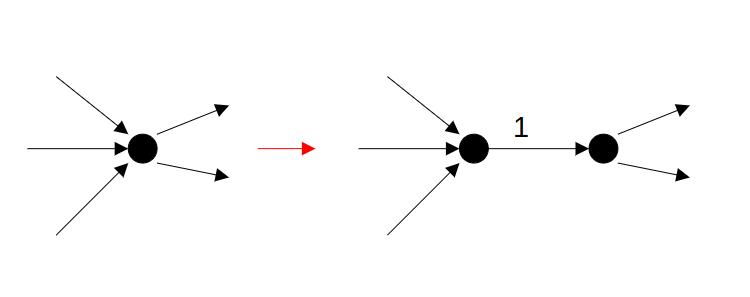
\includegraphics[width=0.4\textwidth]{data/zad43.png}
	\caption{  }
	\label{fig:zad43_fig}
\end{figure}

Wywołujemy Forda-Fulkersona na grafie $G'$, który zwróci nam 
wartość maksymalnego przepływu oraz przepływ $f$. Aby zapisać ścieżki
tworzymy graf $G''$, w którym usuwamy wszystkie krawędzie $e \in E(G)$,
tż., $f(e) = 0$. Dla każdego sąsiada $v$ idziemy do $w$, odkładając
napotkane wierzchołki do na listę. Zwracamy wszystkie listy. 

\subsection{Zadanie 4 -- Znajdowanie najmniejszego przekroju w sieci}
\textbf{Treść: } Przekrojem sieci $(G, c, s, t)$ 
nazywamy podział zbioru $V(G)$ na 
rozłączne zbiory $S$ i $T$ taki, że $s \in S$
oraz $t \in T$. Przepustowość takiego przekroju to suma
$\sum_{v\in S,w\in T} c(vw)$.
Zaprojektuj algorytm, który znajdzie przekrój 
o najmniejszej przepustowości w danej sieci przepływowej.

\textbf{Rozwiązanie: }
Rozwiązanie polega na uruchomieniu algorytmu Floyda-Fulkersona, a
następnie przebadaniu sieci rezydualnej $R$ dla maksymalnego przepływu $f$
zwróconego przez ten algorytm.

Uruchamiamy DFS lub BFS w celu znalezienia wszystkich osiągalnych wierzchołków 
z $s$ w sieci rezydualnej $R$. Zbiór osiągalnych wierzchołków $S$ oraz 
$\overline{S} = V(G) \setminus S$ stanowią podział o najmniejszej 
przepustowości.

\subsection{Zadanie 5 -- Algorytm Dinic'a}
\textbf{Treść: } Niech $R$ będzie siecią rezydualną 
dla pewnej sieci przeplywowej $(G, c, s, t)$ i przepływu $f$; 
niech $d$ będzie
odległością (w sensie liczby krawędzi) od $s$ do $t$ w $R$. 
Przez przeplyw blokujący w $R$ rozumiemy przepływ $f'$ w R taki,
że każda ścieżka od $s$ do $t$ w $f'$ ma dokładnie 
$d$ krawędzi oraz dla każdej ścieżki o $d$ krawędziach od $s$ do $t$ w $R$,
przynajmniej jedna krawędź tej ścieżki jest nasycona przez $f'$.
\begin{itemize}
	\item[a)] Zaprojektuj algorytm, który znajdzie przepływ blokujący w czasie $O(nm)$
	\item[b)] Skonstruuj algorytm rozwiązujący problem maksymalnego przepływu w czasie $O(n^2m)$
\end{itemize}
\textbf{Rozwiązanie: }

\begin{defi}
	Niech $R$ będzie siecią rezydualną dla pewnej sieci przepływowej
	$(G, c, s, t)$ oraz przepływu $f$. Niech $d$ będzie odległością w sensie
	liczby krawędzi od $s$ do $t$ w $R$.
	
	Przez przepływ blokujący w $R$ rozumiemy przepływ $b$ w sieci
	$(R, c_f, s, t)$, taki, że każda ścieżka od $s$ do $t$ 
	w $b$ ma dokładnie $d$ krawędzi oraz dla każdej ścieżki o $d$ 
	krawędziach od $s$ do $t$ w $R$, przynajmniej jedna krawędź tej ścieżki
	jest nasycona przez $b$.
\end{defi}

BFS + usuwanie niepotrzebnych krawędzi w $R$ w celu utworzenia tzw. 
grafu warstwowego, potem DFS w celu przejscia po kazdej ścieżce
i utworzenia przepływów.
\textbf{Rozwiązanie b: }

\begin{algorithm}[H]
	\caption{Algorytm Dinic'a}
	\begin{algorithmic}[1]
		\Procedure{Dinic($G, w$, $s$, $t$)}{}
		\State Niech $f$ to zerowy przepływ w sieci $(G,c,s,t)$
		\State Utwórz sieć rezydualną $(R, c_f)$ dla wejściowej 
		sieci przepływowej oraz dla $f$ 
		\While{Istnieje ścieżka powiększająca w $R$}
		\State Znajdź przepływ blokujący $f'$ w sieci ($R, c_f$, $s$, $t$)
		\State Powiększ $f$ o $f'$
		\State Uaktualnij $(R, c_f)$
		\EndWhile
		\State \Return $f$
		\EndProcedure
	\end{algorithmic}
	\label{zad45}
\end{algorithm}

\subsection{Zadanie 6 -- Wyznaczanie pesymistycznej wydajności w sieci}
\textbf{Treść: } Przypuśćmy, że mamy daną sieć przewodową składającą 
się z $n$ węzłów (w tym jeden serwer) i $m$
połączeń między węzłami, przy czym każde połączenie ma pewną 
przepustowość wyrażoną w kB/s. Zakładamy, że
każdy węzeł może jedynie odbierać dane i przesyłać je 
dalej (w szczególności, zabronione są modyfikacje danych przed
ich przesłaniem). Przez pesymistyczną wydajność sieci 
rozumiemy najwiekszą wartość $w$ taką, że serwer jest w stanie
wysyłać jednocześnie do każdego innego węzła dane w ilości $w$ kB/s.

Zaprojektuj algorytm, który wyznaczy pesymistyczną wydajność zadanej sieci.

\textbf{Rozwiązanie: }
Rozwiązanie polega na połączeniu wszystkich routerów z ujściem $t$ krawędziami 
o przepustowości 1. Jeżeli po wywołaniu algorytmu znajdującego maksymalny
przepływ każda z krawędzi do ujścia $t$ jest nasycona, to 
zwiększamy przepustowość każdej z tych krawędzi o 1 i ponawiamy próbę.
Ostatnia liczba dla której wszysktkie krawędzie były nasycone to 
szukane $w$.


Powyższe rozumowanie można zoptymalizować korzystając z 
binarnego przeszukiwania. Jako maximum przyjmujemy
sumę przepustowości na krawędziach
wychodzących z $s$ 
(bo $\text{val} f_max$ jest nie większe niż
wartość dowolnego przekroju), a jako minimum - 1.

\begin{algorithm}[H]
	\caption{Wyznaczanie pesymistycznej wydajności}
	\begin{algorithmic}[1]
		\Procedure{FindPesimisticEfficiency($G, c$, $s$)}{}
		\State Niech $V' = V(G) + \{t\}$
		\State Niech $E' = E(G) + \{vt : v \in V' \setminus \{s, t\} \}$
		\State Niech $G' = (V', E')$
		\State $R \gets \sum_{v \in N(s)}c(sv)$
		\State $L \gets 1$
		\While{$L < R$}
		\State $w = \lfloor \frac{L + R}{2} \rfloor$
		\For{$e \in E'$}
		\State $c(e) = w$
		\EndFor 
		\State $f \gets$ Ford-Fulkerson($G'$, $c$, $s$, $t$)
		\If{$\forall_{e \in E'} f(e) = w$}
		\State $L \gets w + 1$
		\Else
		\State $R \gets w - 1$
		\EndIf
		\EndWhile
		\State \Return $w$
		\EndProcedure
	\end{algorithmic}
	\label{zad46}
\end{algorithm}

\subsection{Zadanie 8}
\textbf{Treść:} Rozważmy pociąg, który zatrzymuje się na stacjach 
numerowanych liczbami od 1 do $n$. Pociag może
przewozić jednocześnie P pasażerów. Dla każdej pary stacji 
$i$, $j$, gdzie $i < j$, mamy daną liczbę $b_{ij}$ pasażerów chcących
przejechać od stacji $i$ do $j$ oraz koszt jednego takiego biletu $c_ij$ .
Zaprojektuj algorytm, który określi, komu należy sprzedać bilety tak, 
aby zmaksymalizować zysk (tzn. sumę kosztów
sprzedanych biletów).
\section{Algorytmy z nawrotami (backtracking)}

\end{document}